% Options for packages loaded elsewhere
% Options for packages loaded elsewhere
\PassOptionsToPackage{unicode}{hyperref}
\PassOptionsToPackage{hyphens}{url}
\PassOptionsToPackage{space}{xeCJK}
%
\documentclass[
  12pt,
]{scrartcl}
\usepackage{xcolor}
\usepackage[left=1in,right=1in,top=1in,bottom=1in]{geometry}
\usepackage{amsmath,amssymb}
\setcounter{secnumdepth}{3}
\usepackage{iftex}
\ifPDFTeX
  \usepackage[T1]{fontenc}
  \usepackage[utf8]{inputenc}
  \usepackage{textcomp} % provide euro and other symbols
\else % if luatex or xetex
  \usepackage{unicode-math} % this also loads fontspec
  \defaultfontfeatures{Scale=MatchLowercase}
  \defaultfontfeatures[\rmfamily]{Ligatures=TeX,Scale=1}
\fi
\usepackage{lmodern}
\ifPDFTeX\else
  % xetex/luatex font selection
  \setmainfont[]{Crimson}
  \ifXeTeX
    \usepackage{xeCJK}
    \setCJKmainfont[]{Noto Serif KR}
  \fi
  \ifLuaTeX
    \usepackage[]{luatexja-fontspec}
    \setmainjfont[]{Noto Serif KR}
  \fi
\fi
% Use upquote if available, for straight quotes in verbatim environments
\IfFileExists{upquote.sty}{\usepackage{upquote}}{}
\IfFileExists{microtype.sty}{% use microtype if available
  \usepackage[]{microtype}
  \UseMicrotypeSet[protrusion]{basicmath} % disable protrusion for tt fonts
}{}
\makeatletter
\@ifundefined{KOMAClassName}{% if non-KOMA class
  \IfFileExists{parskip.sty}{%
    \usepackage{parskip}
  }{% else
    \setlength{\parindent}{0pt}
    \setlength{\parskip}{6pt plus 2pt minus 1pt}}
}{% if KOMA class
  \KOMAoptions{parskip=half}}
\makeatother
% Make \paragraph and \subparagraph free-standing
\makeatletter
\ifx\paragraph\undefined\else
  \let\oldparagraph\paragraph
  \renewcommand{\paragraph}{
    \@ifstar
      \xxxParagraphStar
      \xxxParagraphNoStar
  }
  \newcommand{\xxxParagraphStar}[1]{\oldparagraph*{#1}\mbox{}}
  \newcommand{\xxxParagraphNoStar}[1]{\oldparagraph{#1}\mbox{}}
\fi
\ifx\subparagraph\undefined\else
  \let\oldsubparagraph\subparagraph
  \renewcommand{\subparagraph}{
    \@ifstar
      \xxxSubParagraphStar
      \xxxSubParagraphNoStar
  }
  \newcommand{\xxxSubParagraphStar}[1]{\oldsubparagraph*{#1}\mbox{}}
  \newcommand{\xxxSubParagraphNoStar}[1]{\oldsubparagraph{#1}\mbox{}}
\fi
\makeatother


\usepackage{longtable,booktabs,array}
\usepackage{calc} % for calculating minipage widths
% Correct order of tables after \paragraph or \subparagraph
\usepackage{etoolbox}
\makeatletter
\patchcmd\longtable{\par}{\if@noskipsec\mbox{}\fi\par}{}{}
\makeatother
% Allow footnotes in longtable head/foot
\IfFileExists{footnotehyper.sty}{\usepackage{footnotehyper}}{\usepackage{footnote}}
\makesavenoteenv{longtable}
\usepackage{graphicx}
\makeatletter
\newsavebox\pandoc@box
\newcommand*\pandocbounded[1]{% scales image to fit in text height/width
  \sbox\pandoc@box{#1}%
  \Gscale@div\@tempa{\textheight}{\dimexpr\ht\pandoc@box+\dp\pandoc@box\relax}%
  \Gscale@div\@tempb{\linewidth}{\wd\pandoc@box}%
  \ifdim\@tempb\p@<\@tempa\p@\let\@tempa\@tempb\fi% select the smaller of both
  \ifdim\@tempa\p@<\p@\scalebox{\@tempa}{\usebox\pandoc@box}%
  \else\usebox{\pandoc@box}%
  \fi%
}
% Set default figure placement to htbp
\def\fps@figure{htbp}
\makeatother


% definitions for citeproc citations
\NewDocumentCommand\citeproctext{}{}
\NewDocumentCommand\citeproc{mm}{%
  \begingroup\def\citeproctext{#2}\cite{#1}\endgroup}
\makeatletter
 % allow citations to break across lines
 \let\@cite@ofmt\@firstofone
 % avoid brackets around text for \cite:
 \def\@biblabel#1{}
 \def\@cite#1#2{{#1\if@tempswa , #2\fi}}
\makeatother
\newlength{\cslhangindent}
\setlength{\cslhangindent}{1.5em}
\newlength{\csllabelwidth}
\setlength{\csllabelwidth}{3em}
\newenvironment{CSLReferences}[2] % #1 hanging-indent, #2 entry-spacing
 {\begin{list}{}{%
  \setlength{\itemindent}{0pt}
  \setlength{\leftmargin}{0pt}
  \setlength{\parsep}{0pt}
  % turn on hanging indent if param 1 is 1
  \ifodd #1
   \setlength{\leftmargin}{\cslhangindent}
   \setlength{\itemindent}{-1\cslhangindent}
  \fi
  % set entry spacing
  \setlength{\itemsep}{#2\baselineskip}}}
 {\end{list}}
\usepackage{calc}
\newcommand{\CSLBlock}[1]{\hfill\break\parbox[t]{\linewidth}{\strut\ignorespaces#1\strut}}
\newcommand{\CSLLeftMargin}[1]{\parbox[t]{\csllabelwidth}{\strut#1\strut}}
\newcommand{\CSLRightInline}[1]{\parbox[t]{\linewidth - \csllabelwidth}{\strut#1\strut}}
\newcommand{\CSLIndent}[1]{\hspace{\cslhangindent}#1}



\setlength{\emergencystretch}{3em} % prevent overfull lines

\providecommand{\tightlist}{%
  \setlength{\itemsep}{0pt}\setlength{\parskip}{0pt}}



 


\addtokomafont{disposition}{\rmfamily}
\setkomafont{pageheadfoot}{\normalfont\normalcolor\footnotesize}
\setkomafont{pagenumber}{\normalfont\normalcolor\footnotesize}
\usepackage{tocbibind}  % Include TOC, List of Figures, and List of Tables in the TOC
\usepackage{fontspec}    % Ensure font support
% \usepackage{placeins}
% \usepackage{float}
\usepackage{setspace}
\usepackage{indentfirst}
\usepackage{chngcntr}
\counterwithin{figure}{section}
\counterwithin{table}{section}
\usepackage{gb4e} \noautomath
\usepackage{amsmath}
\usepackage{pdflscape}
\usepackage{lipsum}
\usepackage{booktabs}
\usepackage{longtable}
\usepackage{array}
\usepackage{multirow}
\usepackage{wrapfig}
\usepackage{float}
\usepackage{colortbl}
\usepackage{pdflscape}
\usepackage{tabu}
\usepackage{threeparttable}
\usepackage{threeparttablex}
\usepackage[normalem]{ulem}
\usepackage{makecell}
\usepackage{xcolor}
\makeatletter
\@ifpackageloaded{caption}{}{\usepackage{caption}}
\AtBeginDocument{%
\ifdefined\contentsname
  \renewcommand*\contentsname{Table of contents}
\else
  \newcommand\contentsname{Table of contents}
\fi
\ifdefined\listfigurename
  \renewcommand*\listfigurename{List of Figures}
\else
  \newcommand\listfigurename{List of Figures}
\fi
\ifdefined\listtablename
  \renewcommand*\listtablename{List of Tables}
\else
  \newcommand\listtablename{List of Tables}
\fi
\ifdefined\figurename
  \renewcommand*\figurename{Figure}
\else
  \newcommand\figurename{Figure}
\fi
\ifdefined\tablename
  \renewcommand*\tablename{Table}
\else
  \newcommand\tablename{Table}
\fi
}
\@ifpackageloaded{float}{}{\usepackage{float}}
\floatstyle{ruled}
\@ifundefined{c@chapter}{\newfloat{codelisting}{h}{lop}}{\newfloat{codelisting}{h}{lop}[chapter]}
\floatname{codelisting}{Listing}
\newcommand*\listoflistings{\listof{codelisting}{List of Listings}}
\makeatother
\makeatletter
\usepackage{pdflscape}
\makeatother
\makeatletter
\makeatother
\makeatletter
\@ifpackageloaded{caption}{}{\usepackage{caption}}
\@ifpackageloaded{subcaption}{}{\usepackage{subcaption}}
\makeatother
\usepackage{bookmark}
\IfFileExists{xurl.sty}{\usepackage{xurl}}{} % add URL line breaks if available
\urlstyle{same}
\hypersetup{
  pdftitle={How Black and White is Language Processing?},
  pdfauthor={ZACHARY NICHOLAS HOUGHTON},
  hidelinks,
  pdfcreator={LaTeX via pandoc}}


\title{How Black and White is Language Processing?}
\usepackage{etoolbox}
\makeatletter
\providecommand{\subtitle}[1]{% add subtitle to \maketitle
  \apptocmd{\@title}{\par {\large #1 \par}}{}{}
}
\makeatother
\subtitle{An Investigation into the Noisy-channel Processing of
Binomials}
\author{ZACHARY NICHOLAS HOUGHTON}
\date{}
\begin{document}
\pagenumbering{roman}
\cleardoublepage
\thispagestyle{plain}
\begin{center}
   \null\vfill
   \textbf{%
      How Black and White is Language Processing?\\
	  An Investigation into the Noisy-channel Processing of Binomials
   }%
   \\
   \bigskip
   By \\
   \bigskip
   {ZACHARY NICHOLAS HOUGHTON}
\\   
   %2020 EDIT: Removed double-spacing btwn name and DISSERTATION   
   %\bigskip
   %B.S. (University of California, Davis) 2001 \\
   %\bigskip
   %2019 EDIT: Removed line for previous degree.
   THESIS \\
   \bigskip
   Submitted in partial satisfaction of the requirements for the
   degree of \\
   \bigskip
   MASTER OF ARTS \\
   \bigskip
   in \\
   \bigskip
   {Psychology} \\ 
      \bigskip
   in the \\
   \bigskip
   OFFICE OF GRADUATE STUDIES \\
   \bigskip        
   of the \\
   \bigskip
   UNIVERSITY OF CALIFORNIA \\
   \bigskip
   DAVIS \\
   \bigskip
   Approved: \\
   \bigskip
   \bigskip
   \makebox[3in]{\hrulefill} \\
   Dr.~Fernanda Ferreira, Chair \\
   \bigskip
   \bigskip
   \makebox[3in]{\hrulefill} \\
   Dr.~Emily Morgan \\
   \bigskip
   \bigskip
   \makebox[3in]{\hrulefill} \\
   Dr.~John Henderson \\
   \bigskip
   Committee in Charge \\
   \bigskip
   2025 \\
   \vfill
\end{center}


\newpage
\newcounter{savedpage}
\setcounter{savedpage}{\value{page}}

\thispagestyle{empty}
\begin{titlepage}
\vspace*{\stretch{1}}
\begin{center}
  Copyright \copyright\ 2025 by Zachary Nicholas Houghton. \\
  \textit{All rights reserved.}
\end{center}
\end{titlepage}

\setcounter{page}{\value{savedpage}} % Reset the counter
\clearpage

\renewcommand*\contentsname{Table of contents}
{
\setcounter{tocdepth}{3}
\tableofcontents
}

\newpage

\doublespacing

\setlength{\parindent}{4em}

\section*{Abstract}\label{sec-abstract}
\addcontentsline{toc}{section}{Abstract}

Abstract

\newpage

\pagenumbering{arabic}

\section{Introduction}\label{introduction}

Humans have a great deal of flexibility when it comes to linearizing our
abstract thoughts into discrete words. For example, to express
uncertainty, I have a variety of options ranging from familiar
expressions such as \emph{I don't know}, to more novel expressions, such
as \emph{to me, it is uncertain}. In other words, when speaking we are
faced with the decision of either accessing a holistically stored
expression or generating a novel expression by combining words using
knowledge of the grammar.

Traditionally, the assumption about this trade off between item-specific
and generative knowledge was thought to be a function of a word or
phrase's semantic compositionally {[}i.e., the degree to which the
phrase's meaning could be derived from the individual words or morphemes
that comprise it; Chomsky
(\citeproc{ref-chomskyAspectsTheorySyntax1965}{1965}); Pinker \& Ullman
(\citeproc{ref-pinkerFutureTense2002}{2002}){]}. For example, according
to generativist theories, regular multi-morphemic words can be composed
using rules of the language. As such, a word like \emph{cats} would be
generated by accessing the holistically stored word, \emph{cat}, and
then generating \emph{cats} by using knowledge of the grammar with
respect to plural formation. Similarly, multi-word phrases, such as
\emph{I don't know} would be generated by accessing each of the
individual words in the phrase and then combining them.

These theories gained a great deal of traction, partially due to
concerns about memory limitations. However, more recently we have
learned that the brain has a much larger memory capacity than we once
thought. For example, Wang et al.
(\citeproc{ref-wangDiscoveringCapacityHuman2003}{2003}) demonstrated
that the human brain can store an upwards of 10\textsuperscript{8432}
bits. Further, Mollica \& Piantadosi
(\citeproc{ref-mollicaHumansStoreMegabytes2019}{2019}) estimated that
the upper bound of memory that it would require to store linguistic
knowledge is ten million bits of information, which is well within the
estimated amount of storage that the human brain has.

As knowledge of the memory capacity of the brain increased, alternative
accounts to holistic storage started gaining traction. These theories
grew largely out of the phonetics and categorization literature where
generativists' cookie-cutter approach to language was easily shown to
fall short. For example, Bybee
(\citeproc{ref-bybeeWordFrequencyContext2002}{2002}) demonstrated that
the phonetic reduction of a sound advances more greatly in
high-frequency words than low-frequency words. If words are the
combination of abstract phonemes, then the reduction of a phoneme should
proliferate across every word that contains the phoneme. In other words,
it's hard to account for the context-specificity of phoneme realizations
without a storage mechanism that contains context-specific phonetic
detail.

Similarly, McMurray et al.
(\citeproc{ref-mcmurrayGradientSensitivityWithincategory2008}{2008}) in
their seminal paper demonstrated that people are sensitive to gradient
changes of within-category voice onset timing (VOT). VOT is a measure of
when the vocal chords begin flapping. While VOT is a continuous measure,
it is used by English listeners to determine whether a sound is voiced
or unvoiced. Following this, if phonemes are represented as abstract
categories (e.g., just \emph{p} or \emph{b}), then VOT should only
influence listener's perception if the change in VOT results in a change
in the phoneme. That is, if two sounds vary in VOT but are still
classified as \emph{p}, participants should not be sensitive to this (if
they're decomposing the word into abstract phoneme units). However,
McMurray et al.
(\citeproc{ref-mcmurrayGradientSensitivityWithincategory2008}{2008})
demonstrated that listeners \emph{are} sensitive to within-category VOT.
Specifically, they presented participants with words such as
\emph{barricade/parakeet}, where the initial sounds were either voiced
or voiceless stops. They then systematically manipulated the VOT for the
initial stop and measured the proportion of participants' fixations to
the competitor. They found that within-category variability of VOT
affected participants' proportion of fixations to the competitor,
suggesting sensitivity to within-category variability in VOT.

These findings also sparked similar questions in the word-processing
literature. For example, Bybee \& Scheibman
(\citeproc{ref-bybeeEffectUsageDegrees1999}{1999}) examined the phonetic
reduction of \emph{don't} in various contexts. They found that
\emph{don't} is more greatly reduced in \emph{I don't know} than in
lower-frequency phrases such as \emph{I don't go}. In other words, the
phonetic reduction of \emph{I don't know} cannot be attributed to the
phonetic reduction of any of the individual parts in isolation. This
suggests that \emph{I don't know} has a representation separate from the
individual parts. Bybee \& Scheibman
(\citeproc{ref-bybeeEffectUsageDegrees1999}{1999}) showed similar
results for other high-frequency phrases as well, such as \emph{have
to}, \emph{want to}, etc. Similarly, Yi
(\citeproc{ref-yiEumunHyeonsanggwaBindo2002}{2002}) demonstrated that
tensification in certain multi-word phrases in Korean is also
context-specific. Specifically, in Korean certain consonants become
tense when they occur after the future tense marker. Yi
(\citeproc{ref-yiEumunHyeonsanggwaBindo2002}{2002}) demonstrated that
this tensification is more frequent in high-frequency phrases.

In the Psycholinguistics literature, there has been a rich literature
examining the multi-word holistic storage of binomials
(\citeproc{ref-houghton2023doespredictabilitydrive}{Houghton \& Morgan,
2023},
\citeproc{ref-houghton2024frequencydependentpreferenceextremity}{2024};
\citeproc{ref-morganFormalizingConstructionGrammar}{Morgan, n.d.};
\citeproc{ref-morganModelingIdiosyncraticPreferences2015}{Morgan \&
Levy, 2015}, \citeproc{ref-morganAbstractKnowledgeDirect2016}{2016a},
\citeproc{ref-morganFrequencydependentRegularizationIterated2016a}{2016b},
\citeproc{ref-morganProductiveKnowledgeItemspecific2024}{2024};
\citeproc{ref-siyanova-chanturiaSeeingPhraseTime2011}{Siyanova-Chanturia
et al., 2011}). For example, Siyanova-Chanturia et al.
(\citeproc{ref-siyanova-chanturiaSeeingPhraseTime2011}{2011})
demonstrated that binomials are read faster in their frequent order
(e.g., \emph{bread and butter}) than in their infrequent ordering (e.g.,
\emph{butter and bread}). If binomials were represented and processed
word-by-word then it is unclear how to account for this result since the
individual words are identical. One possibility is that humans have
abstract preferences for ordering words in phrases (e.g., a preference
for short words first). Morgan \& Levy
(\citeproc{ref-morganAbstractKnowledgeDirect2016}{2016a}) examined this
possibility by creating a corpus of binomials and annotating them for
semantic and phonological constraints known to influence binomial
orderings (\citeproc{ref-benorChickenEggProbabilistic2006}{Benor \&
Levy, 2006}). They then created a logistic model to combine these
constraints into a single generative preference value that indicated the
direction and magnitude of the preference. For example, a large
generative preference value indicates a strong preference for the
alphabetical ordering.

They further examined whether human ordering preferences are driven by
these generative preferences for binomials ranging in overall frequency
(where overall frequency is the total number of times a binomial occurs
in either ordering, e.g., the number of times \emph{bread and butter}
occurs plus the number of times \emph{butter and bread} occurs). They
found that for low-frequency binomials, human ordering preferences are
driven primarily by generative preferences, however for high-frequency
binomials human ordering preferences are driven primarily by relative
frequency (i.e., the proportion of counts in the alphabetical ordering
to the nonalphabetical ordering, e.g., the proportion of counts of
\emph{bread and butter} to counts of \emph{butter and bread}). Their
results suggest that humans generate low-frequency binomials using
generative knowledge of the language, however for high-frequency
binomials humans store and access a holistic representation of the
entire binomial.

\subsection{Frequency-dependent Preference
Extremity}\label{frequency-dependent-preference-extremity}

Holistic storage also makes rich predictions about language change that
have been born out in the literature. For example, there is evidence
that ordering preferences become more extreme for high-frequency items
relative to low-frequency items
(\citeproc{ref-liuFrequencydependentRegularizationConstituent2020}{Liu
\& Morgan, 2020},
\citeproc{ref-liuFrequencyDependentRegularizationSyntactic2021}{2021};
\citeproc{ref-morganFrequencydependentRegularizationIterated2016a}{Morgan
\& Levy, 2016b}). If phrases are generated compositionally without any
holistic storage, it is hard to see how high-frequency phrases would
become more polarized, especially binomials since both orderings contain
the same words. However, this is precisely what the literature has
demonstrated. For example, Morgan \& Levy
(\citeproc{ref-morganFrequencydependentRegularizationIterated2016a}{2016b})
demonstrated that the ordering preferences of binomials are more extreme
for high-frequency binomials relative to low-frequency binomials.

Additionally, Liu \& Morgan
(\citeproc{ref-liuFrequencydependentRegularizationConstituent2020}{2020})
demonstrated that the dative alternation (e.g., \emph{give him the ball}
vs \emph{give the ball to him}) also shows evidence of
frequency-dependent preference extremity. Specifically, they found that
for high-frequency verbs, there is a stronger preference for using one
dative alternation over the other than for low-frequency verbs.
Similarly, Liu \& Morgan
(\citeproc{ref-liuFrequencyDependentRegularizationSyntactic2021}{2021})
examined the ordering of adjectives in adjective-adjective-noun (AAN)
phrases (e.g., \emph{dark blue sky}). They found that AAN phrases with
higher overall frequency (where overall frequency is the sum of counts
in either ordering) show more polarized ordering preferences.

While holistic storage is a prerequisite for frequency-dependent
preference extremity, it isn't enough by itself to account for this
phenomenon. In addition to holistic storage, it is possible that
frequency-dependent preference extremity arises as an interaction
between imperfect learning and transmission across generations
(\citeproc{ref-houghton2024frequencydependentpreferenceextremity}{Houghton
\& Morgan, 2024};
\citeproc{ref-morganFrequencydependentRegularizationIterated2016a}{Morgan
\& Levy, 2016b}). This idea was proposed by Morgan \& Levy
(\citeproc{ref-morganFrequencydependentRegularizationIterated2016a}{2016b})
who demonstrated that a frequency-independent regularization bias can
account for frequency-dependent preference extremity arising across
generations of learners.

Specifically they used a 2-alternative iterated learning paradigm
(\citeproc{ref-realiEvolutionFrequencyDistributions2009}{Reali \&
Griffiths, 2009}) to simulate the evolution of binomial ordering
preferences across generations of speakers. In their model, a speaker
first produces N binomial expressions in either ordering in proportion
to their learned preferences. For the first generation of speakers, this
proportion is simply the generative preference of the binomial. The
learner then ``hears'' these Nbinomial expressions and updates their
hypothesis about the proportion that each ordering of that binomial
occurs in. This data generation process alone simply results in
learner's converging on the prior
(\citeproc{ref-griffithsLanguageEvolutionIterated2007}{Griffiths \&
Kalish, 2007}). Thus, Morgan \& Levy
(\citeproc{ref-morganFrequencydependentRegularizationIterated2016a}{2016b})
introduced a frequency-independent regularization bias into their model.
This was a prior that the learner had to overcome. Thus, if there was
enough evidence, learners would develop stronger preferences for the
ordering of a binomial, however, if there was not strong evidence then
the learner's preferences would be overpowered by the prior. This model
resulted in frequency-dependent preference extremity arising across
generations of learners.

However, while their results demonstrate that a frequency-independent
regularization bias can account for frequency-dependent preference
extremity, it's unclear what process this bias is analogous to in
language.

\subsection{Noisy-channel Processing}\label{noisy-channel-processing}

One possibility is that the the frequency-independent regularization
bias is a function of noisy-channel processing.\footnote{It is worth
  mentioning here that in parallel to the development of noisy-channel
  processing theories, other accounts making similar claims also emerged
  (e.g., \citeproc{ref-ferreiraGoodEnoughApproach2007}{Ferreira \&
  Patson, 2007}). Many of these theories accept that language processing
  must allow for flexibility and it's often difficult to disentangle
  them. While we take a noisy-channel approach in the present thesis,
  all of the claims we make are also compatible with good-enough
  processing theories as well, and we leave the task of disentangling
  the two to future work.}

When processing language, we are faced with a great deal of noise in our
environment. This can be literal noise in our environment, such as the
sound of a loud city, or noise introduced by the communication device,
such as static in a cellphone conversation. It can also be errors made
by the speaker (saying the wrong thing) or by the listener (hearing the
wrong thing). Despite this, human's language processing system appears
to be quite robust to noise. One possible explanation is that people may
be tracking, not simply what the speaker is saying, but what probable
utterances the speaker \emph{could} say
(\citeproc{ref-gibsonNoisyChannelAccountCrosslinguistic2013}{Gibson et
al., 2013}; \citeproc{ref-levyNoisychannelModelHuman2008}{Levy, 2008}).

There is a great deal of evidence that people do take noise into
account. First and most obviously, when a listener misses a word due to
simply not hearing it, it very rarely causes a complete breakdown in
communication. Further, Ganong
(\citeproc{ref-ganongPhoneticCategorizationAuditory1980}{1980})
demonstrated that people process a non-word as being a word under noisy
conditions. Similarly, Felty et al.
(\citeproc{ref-feltyMisperceptionsSpokenWords}{n.d.}) found that when
listeners misperceive a word, the word that they believed to have heard
is a higher frequency than the word spoken. These results suggest that
in noise listeners are relying on information about the language, such
as what utterances are more probable.

Interestingly, people will sometimes even hear a grammatical sentence
and interpret the meaning differently from what they have heard due to
noisy-channel processing. For example Christianson et al.
(\citeproc{ref-christiansonThematicRolesAssigned2001}{2001}) found that
when people read the sentence \emph{While the man hunted the deer ran
into the woods}, people will answer in the affirmative for the question
\emph{Did the man hunt the deer?} as well as the question \emph{Did the
deer run into the woods?}. Levy
(\citeproc{ref-levyNoisychannelModelHuman2008}{2008}) argued that since
both interpretations can arise from a single insertion, noisy-channel
processing offers an explanation for this finding.

Following this, Gibson et al.
(\citeproc{ref-gibsonNoisyChannelAccountCrosslinguistic2013}{2013})
formalized noisy-channel processing using a Bayesian framework. They
modeled noisy-channel processing as a process wherein the listener
estimates the probability of the speaker's intended utterance (\(s_i\))
given what they perceived (\(s_p\), Equation~\ref{eq-gibsonnoisy})
Specifically, the listener is modeled as a rational Bayesian who
estimates the probability of the speaker's intended utterance given the
perceived utterance as being proportional to the probability of the
intended utterance in general times the probability of that perceived
utterance given the intended utterance. This is formalized
mathematically in Equation~\ref{eq-gibsonnoisy} where \(s_i\) is the
speaker's intended sentence and \(s_p\) is the perceived sentence. The
prior (\(P(s_p|s_i)\)) is the likelihood of the \(s_i\) being corrupted
to \(s_p\).

\begin{equation}\phantomsection\label{eq-gibsonnoisy}{
P(s_i|s_p)\propto P(s_i) P(s_p|s_i) 
}\end{equation}

The model in Gibson et al.
(\citeproc{ref-gibsonNoisyChannelAccountCrosslinguistic2013}{2013}) made
several predictions. Specifically, their model predicted that
comprehenders should be more likely to interpret a semantically
implausible sentence (e.g., \emph{the mother gave the candle the
daughter}) as being plausible (e.g., \emph{the mother gave the candle to
the daughter}) if there is increased noise (which they accomplished by
adding syntactic errors to the filler items). Their model also predicted
that increasing the probability of an implausible utterance (e.g., by
adding more implausible items to the fillers) should lead to an
increased rate of implausible interpretations. They tested these
predictions by giving participants a series of sentences, some of which
were semantically implausible but had semantically plausible
alternatives that participants could interpret the sentence as being.
These alternatives varied in how different they were from the perceived
utterances. Some of them varied from the perceived utterance by a single
insertion or a single deletion, while others varied by two insertions or
two deletions. By manipulating the number of semantically implausible
sentences as well as the number of filler items with syntactic errors,
both of the predictions that their model made were born out.

Given these results, Houghton \& Morgan
(\citeproc{ref-houghton2024frequencydependentpreferenceextremity}{2024})
extended Morgan \& Levy
(\citeproc{ref-morganFrequencydependentRegularizationIterated2016a}{2016b})'s
model. Specifically, we used a 2-alternative iterated learning paradigm,
learners heard N tokens of a given binomial in either alphabetical or
nonalphabetical order and learns a preference. The learner's goal was to
learn the ordering preferences for each binomial. Then after learning
the ordering preferences, they then produced N tokens to the next
generation. This process then repeats.

Specifically, after hearing a binomial, the learner in our model updated
their beliefs in proportion to what they believed the speaker's intended
ordering was, which was modeled with pseudo counts. For example, if they
believed the intended utterance was A and B with 60\% probability and B
and A with 40\% probability, then they would add 0.6 and 0.4 to the
pseudo counts for A and B and B and A respectively.\footnote{See
  Houghton \& Morgan
  (\citeproc{ref-houghton2024frequencydependentpreferenceextremity}{2024})
  for a more detailed explanation of our computational model.} These
updated beliefs would result in the learner prescribing an even higher
probability of A and B occurring.

Without a regularization bias, this model would simply result in
convergence to the prior
(\citeproc{ref-griffithsLanguageEvolutionIterated2007}{Griffiths \&
Kalish, 2007}). Thus, our model also contained a noisy-channel
processing component. After hearing a binomial, the learner in our model
would interpret the opposite ordering occasionally (following
Equation~\ref{eq-gibsonnoisy}). That is, if the learner hears B and A,
but is confident that the intended ordering was actually A and B, they
will update their beliefs as if they had heard A and B.

To help build intuition for this: suppose a learner believes there is a
60\% chance that the speaker intended to say A and B, but they heard B
and A. Without a noisy-channel processing component, the learner would
update their belief, down-weighting the probability of A and B and
up-weighting the probability of B and A. However, with noisy-channel
processing, the learner may actually assume the speaker intended to say
A and B (after calculating this probability according to
Equation~\ref{eq-gibsonnoisy}). This would then result in updating their
beliefs as if they had heard A and B. For high-frequency binomials, the
learner may be quite confident about their expectations for the ordering
of the binomial, and may be more willing to interpret B and A as A and
B. However, for low-frequency binomials, the learner may be less
confident and restrain from interpreting B and A as A and B.

Indeed, this is precisely the result we found in Houghton \& Morgan
(\citeproc{ref-houghton2024frequencydependentpreferenceextremity}{2024}).
That is, that for low-frequency binomials, the learner's belief about
the intended ordering was not particularly strong and was pulled towards
the prior. However, for high-frequency binomials, as the learning
continued iteratively across generations, frequency-dependent preference
extremity arose.

Our results in Houghton \& Morgan
(\citeproc{ref-houghton2024frequencydependentpreferenceextremity}{2024})
demonstrated that a noisy-channel processing model in an iterative
learning paradigm can predict frequency-dependent preference extremity.
It also makes a crucial prediction: that learners sometimes hear \emph{B
and A}, but actually interpret it to be \emph{B and A}. In the present
study we explore this prediction.

\subsection{Present Thesis}\label{present-thesis}

Houghton \& Morgan
(\citeproc{ref-houghton2024frequencydependentpreferenceextremity}{2024})'s
model predicts that learners sometimes hear one binomial ordering but
interpret it to be the opposite ordering. If this is the case, then it
is possible that upon hearing, e.g., \emph{white and black}, the
listener actually processes it as \emph{black and white}. If this is the
case, then hearing \emph{white and black} should actually speed up the
processing of \emph{black and white} more than it speeds up the
processing of \emph{white and black}. This is the prediction that we set
out to text in the present study. By using a primed self-paced reading
task with a mental rotation task, we examine whether \emph{white and
black} primes \emph{black and white} more than it primes \emph{white and
black}.

\section{Methods}\label{methods}

\subsection{Procedure}\label{procedure}

In order to examine the effects of noisy-channel processing on the
reading times of binomials, we used a primed self-paced reading task
with a mental rotation task. Specifically, participants were first
presented auditorily with a prime sentence while simultaneously
completing a mental rotation task. The mental rotation task involved
determining whether one was a simple rotation or a mirror image of
another image. The rotation was always wither 0 degrees or 45 degrees.
Participants were tasked with either pressing the `f' key or the `j' key
(counter balanced between participants) to indicate that the image was
either a simple rotation or a mirror image. The idea behind the mental
rotation task was that by forcing participants to multi-task they may
rely more on noisy-channel processing than when they can focus solely on
the prime sentences.

After listening to the prime sentence and completing the mental
rotation, participants then completed a self-paced reading task.
Specifically, participants were presented with a sentence word-by-word
and pressed the `space' key when they were ready to proceed to the next
word. Reaction times for the time it took participants to press the
`space' key were recorded for each word. After each sentence,
participants were presented with a comprehension question to test their
attention. The comprehension questions were questions either about the
prime sentence or the sentence they had just read.

\subsection{Stimuli}\label{stimuli}

Our stimuli consisted of 30 polarized binomials.\footnote{Our stimuli
  and analyses are available at the following link:
  \url{https://github.com/znhoughton/Noisy-Channel-Binomial-Preferences}.
  The stimuli are also included in the appendix section
  (Section~\ref{sec-full-list-of-stimuli}).} Specifically, these were
binomials that occurred more than 400,000 times (out of 323,592,921,465
tokens), calculated using the Google \emph{n}-grams corpus
(\citeproc{ref-michel2011quantitativeanalysisculture}{Michel et al.,
2011}). Additionally, they all had a relative frequency of either less
than -0.30 and greater than 0.30. Relative frequency indicates which
ordering is more preferred (and to what magnitude). For example, a
binomial that occurs equally as many times in both orders would have a
relative frequency of zero (where relative frequency ranges from -0.50
to 0.50). A relative frequency value below 0 indicates that the
nonalphabetical ordering occurred more than the alphabetical ordering in
corpus data, and a number above zero indicates the opposite. The
magnitude of the number indicates the strength, with 0.50 indicating
that the binomial occurred exclusively in alphabetical ordering and
-0.50 indicated the binomial occurred exclusively in nonalphabetical
ordering.

For each of these binomials, we created a prime and a target sentence
containing the binomial in either order. Specifically, for each
binomial, three prime sentences were made: one that contained the
binomial in the frequent ordering (e.g., \emph{bread and butter}), one
that contained the infrequent ordering, (\emph{butter and bread}), and
one that did not contain a binomial at all. These priming conditions are
referred to as the frequent, infrequent, and unrelated primes
respectively. We also made two target sentences (the sentences read
during the self-paced reading task) for each binomial. The target
sentences contained the binomial in either the frequent or infrequent
ordering. Finally, we also included 30 filler trials, which did not
contain binomials in the prime or target sentences.

Our prime and target sentences were crossed such that each target
occurred with each prime, however no participant was presented with the
same binomial in more than one trial.

\subsection{Participants}\label{participants}

228 University of California, Davis undergraduate students were given
course credit to participate in the study. We also recruited an
additional 220 participants through Prolific. Altogether, 448 people
participated in our study.

Participants were randomly presented with one of 6 conditions. Since our
design is a 3 x 2 design, 6 conditions were created so that participants
did not encounter the same binomial in more than one trial.

\subsection{Analysis}\label{analysis}

We divided the sentences into a target and spillover region to be our
region of analysis. This region included the 3 words in the binomial
along with the 3 following words. We then excluded participants whose
reading times on this region were less than 100ms or greater than 5000
ms (following \citeproc{ref-morganAbstractKnowledgeDirect2016}{Morgan \&
Levy, 2016a}). We also excluded participants who had an average accuracy
below 0.7 on the audio comprehension questions (the questions that asked
about the auditorily presented prime). Finally, we excluded trials for
which the residual reading times were outside of 2.5 standard deviations
from the mean.

We then ran two Bayesian mixed-effects regression models with residual
reading times as the dependent variable.\footnote{A pre-registration of
  our study is available at the following link:
  \url{https://aspredicted.org/t324-swgk.pdf}.}

For the first model, we were interested in whether a frequent prime
affected the residual reading times. As such, we filtered the dataframe
to include trials that contained either an unrelated or frequent prime.
We then treatment coded our variables such that for the prime sentences,
0 indicated an unrelated prime and 1 indicated a frequent prime. For
target sentences, 0 indicated an infrequent target while 1 indicated a
frequent target. We then ran a model with residual reading time as the
dependent variable, fixed-effects for prime, target, and their
interaction, as well as maximal random-effects (following
\citeproc{ref-barrRandomEffectsStructure2013}{Barr et al., 2013}).

Our second model was similar, however we were interested in how the
infrequent prime affected residual reading times. As such, we filtered
our dataframe to include trials that contained either the unrelated or
infrequent prime. We then treatment coded our variables such that 0
indicated an unrelated prime and 1 indicated an infrequent prime.

Our model syntax was the same for both models, as mentioned previously
the difference was the levels of the variables included in the data.

\begin{equation}\phantomsection\label{eq-models}{
\begin{aligned}
\text{Residual Reading Time} & \sim \text{Intercept} + \text{prime freq} * \text{target freq} \\ 
&+ (\text{prime freq} * \text{target freq} | \text{Item}) + (\text{prime freq} * \text{target freq} | \text{participant})
\end{aligned}
}\end{equation}

\section{Results}\label{results}

We first examined whether a frequent prime facilitated the reading of
the frequent ordering of the binomial more than the reading time of the
infrequent ordering. Following Houghton et al.
(\citeproc{ref-houghtonTaskdependentConsequencesDisfluency2024}{2024}),
in addition to reporting the estimates we also report the percentage of
posterior samples greater than zero. Bayesian statistics don't force us
into a binary interpretation of significance or non-significance, by
reporting the percentage of posterior samples greater than zero we are
able to interpret the results in a more nuanced manner.

The results are presented in Table~\ref{tbl-frequentresults} and
visualized in Figure~\ref{fig-fullresults}. Since prime and target types
were treatment coded, the Intercept represents the estimated reading
times for unrelated prime sentences with an infrequent target sentence.
Coefficient estimates represent the distance from the Intercept.
Although the credible interval crosses zero, over 93\% of the posterior
samples for the effect of frequent prime were greater than zero,
suggesting that for not-frequent targets, the frequent prime resulted in
slower reading times than the unrelated prime. Similarly, over 93\% of
the posterior samples for frequent target were less than zero,
suggesting that for unrelated primes, the frequent target was read
faster. Finally, about 90\% of the samples for the interaction effect
were less than zero, suggesting that the difference between the reading
times in the unrelated prime condition and the reading times in the
frequent prime condition were larger for infrequent targets than
frequent targets. In other words, the frequent prime speeds up the
reading times for the frequent ordering of the binomial more than the
infrequent ordering of the binomial.

\begin{table}

\caption{\label{tbl-frequentresults}Results of the statistical model for
the frequent vs unrelated prime.}

\centering{

\centering\begingroup\fontsize{11}{13}\selectfont

\begin{tabular}{>{\raggedright\arraybackslash}p{14em}rrrrr}
\toprule
\textbf{ } & \textbf{Estimate} & \textbf{Est.Error} & \textbf{Q2.5} & \textbf{Q97.5} & \textbf{\% Samples > 0}\\
\midrule
\textbf{\cellcolor{gray!6}{Intercept}} & \cellcolor{gray!6}{-169.01} & \cellcolor{gray!6}{20.59} & \cellcolor{gray!6}{-209.40} & \cellcolor{gray!6}{-128.03} & \cellcolor{gray!6}{0.00}\\
\textbf{Frequent Prime} & 25.76 & 17.04 & -7.10 & 59.63 & 93.92\\
\textbf{\cellcolor{gray!6}{Frequent Target}} & \cellcolor{gray!6}{-25.70} & \cellcolor{gray!6}{15.09} & \cellcolor{gray!6}{-56.01} & \cellcolor{gray!6}{3.41} & \cellcolor{gray!6}{4.32}\\
\textbf{Frequent Prime:Frequent Target} & -23.91 & 19.30 & -63.64 & 12.47 & 10.19\\
\bottomrule
\end{tabular}
\endgroup{}

}

\end{table}%

Next we examined whether the infrequent prime speeds up the infrequent
ordering of the binomial more than the frequent ordering. If readers are
engaged in noisy-channel processing when listening to the prime, they
may actually activate \emph{bread and butter} when they hear
\emph{butter and bread}. This would result in the infrequent prime
speeding up the \emph{frequent} ordering of the binomial more than the
infrequent ordering.

The results are presented in Table~\ref{tbl-infrequentresults} and
visualized in Figure~\ref{fig-fullresults}. Similar to the previous
model, since prime and target types were treatment coded, the Intercept
represents the estimated reading times for unrelated prime sentences
with an infrequent target sentence. Coefficient estimates represent the
distance from the Intercept. We find no meaningful main-effect for
infrequent primes or frequent targets, but we do find a meaningful
interaction effect. While the credible interval crosses zero, over 90\%
of the posterior samples were greater than zero. The results suggest
that the infrequent prime speeds up reading for the infrequent target
more than the frequent target.

\begin{table}

\caption{\label{tbl-infrequentresults}Results of the statistical model
for the infrequent vs unrelated prime.}

\centering{

\centering\begingroup\fontsize{11}{13}\selectfont

\begin{tabular}{>{\raggedright\arraybackslash}p{14em}rrrrr}
\toprule
\textbf{ } & \textbf{Estimate} & \textbf{Est.Error} & \textbf{Q2.5} & \textbf{Q97.5} & \textbf{\% Samples > 0}\\
\midrule
\textbf{\cellcolor{gray!6}{Intercept}} & \cellcolor{gray!6}{-173.52} & \cellcolor{gray!6}{20.78} & \cellcolor{gray!6}{-214.07} & \cellcolor{gray!6}{-132.06} & \cellcolor{gray!6}{0.00}\\
\textbf{Infrequent Prime} & 7.48 & 14.00 & -19.71 & 35.31 & 70.50\\
\textbf{\cellcolor{gray!6}{Frequent Target}} & \cellcolor{gray!6}{-13.94} & \cellcolor{gray!6}{14.61} & \cellcolor{gray!6}{-43.68} & \cellcolor{gray!6}{13.84} & \cellcolor{gray!6}{16.81}\\
\textbf{Infrequent Prime:Frequent Target} & 24.57 & 19.39 & -11.57 & 64.51 & 90.53\\
\bottomrule
\end{tabular}
\endgroup{}

}

\end{table}%

\begin{figure}[htbp]

\caption{\label{fig-fullresults}Plot of our results. Points indicate}

\centering{

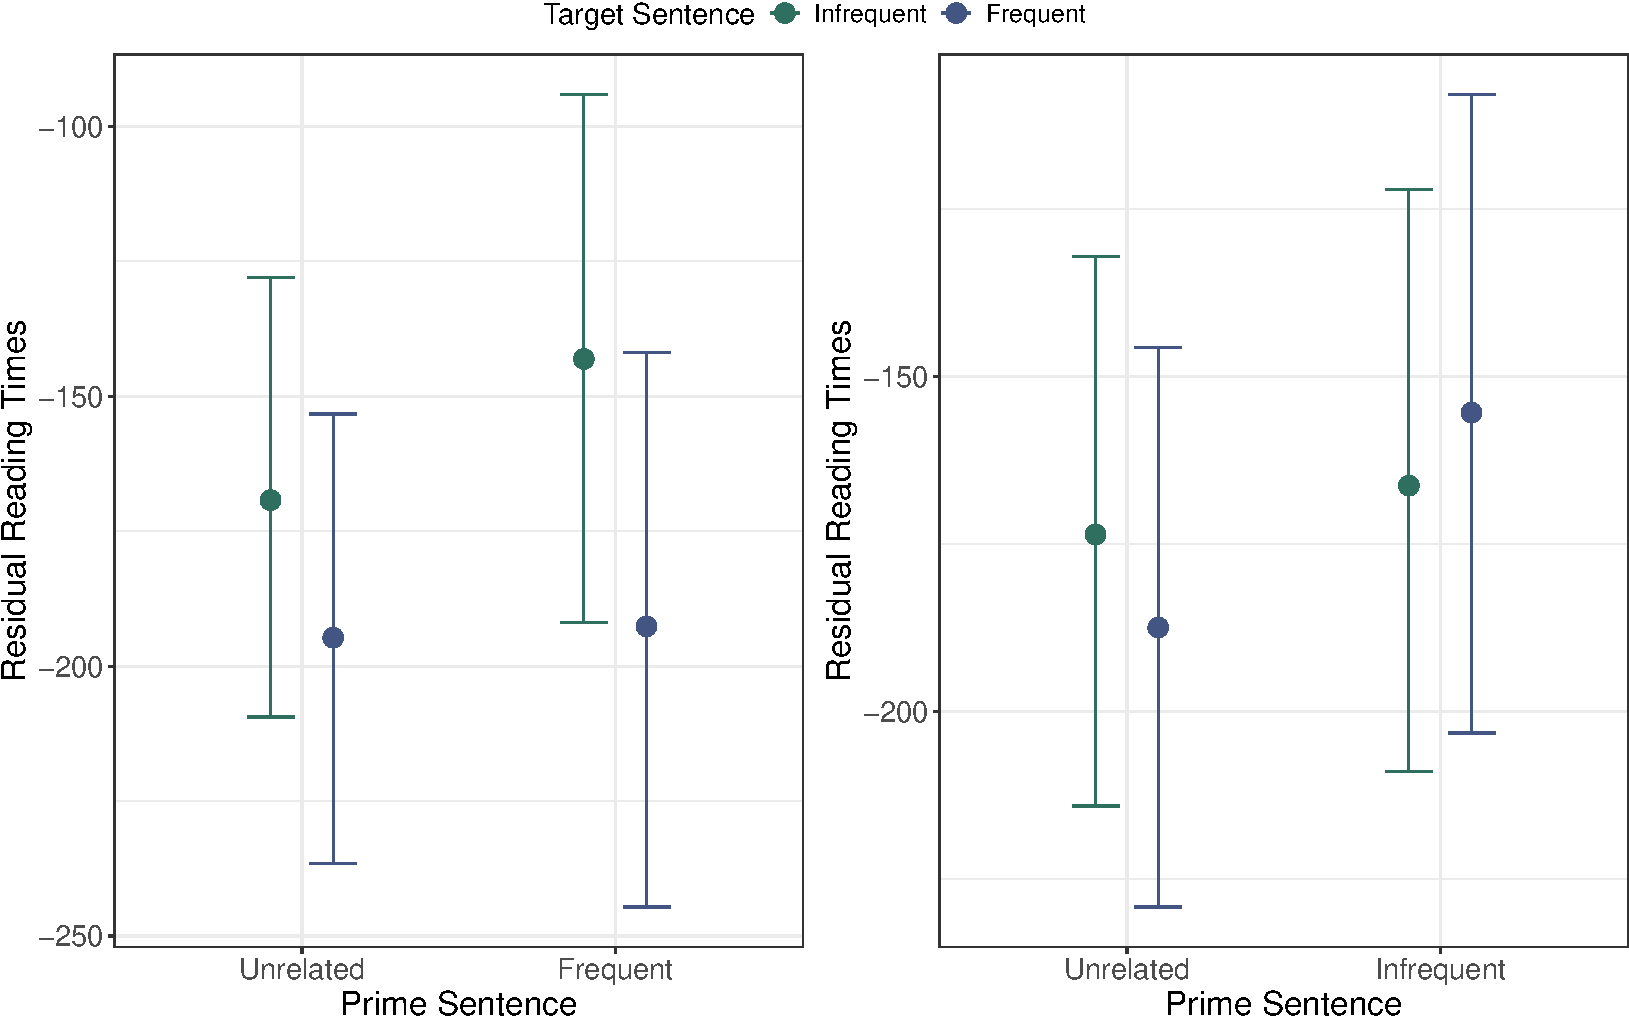
\includegraphics[width=0.8\linewidth,height=\textheight,keepaspectratio]{noisy-channel-binomial-preferences-writeup_files/figure-pdf/fig-fullresults-1.pdf}

}

\end{figure}%

\section{Discussion}\label{discussion}

Our results demonstrate that both the frequent and infrequent ordering
of a given binomial speeds up the reading times of the respective
ordering. That is, priming the frequent ordering speeds up the reading
of the frequent ordering, and priming the infrequent ordering speeds up
the reading of the infrequent ordering.

-Not noisy-channel processing?

-maybe accessibility?

-Still lots of evidence of noisy-channel processing, how to explain?

\clearpage

\section*{References}\label{references}
\addcontentsline{toc}{section}{References}

\phantomsection\label{refs}
\begin{CSLReferences}{1}{0}
\bibitem[\citeproctext]{ref-barrRandomEffectsStructure2013}
Barr, D. J., Levy, R., Scheepers, C., \& Tily, H. J. (2013). Random
effects structure for confirmatory hypothesis testing: Keep it maximal.
\emph{Journal of Memory and Language}, \emph{68}(3), 255--278.
\url{https://doi.org/10.1016/j.jml.2012.11.001}

\bibitem[\citeproctext]{ref-benorChickenEggProbabilistic2006}
Benor, S. B., \& Levy, R. (2006). The chicken or the egg? A
probabilistic analysis of english binomials. \emph{Language},
\emph{82}(2), 233--278. \url{https://doi.org/10.1353/lan.2006.0077}

\bibitem[\citeproctext]{ref-bybeeWordFrequencyContext2002}
Bybee, J. (2002). Word frequency and context of use in the lexical
diffusion of phonetically conditioned sound change. \emph{Language
Variation and Change}, \emph{14}(3), 261--290.
\url{https://doi.org/10.1017/S0954394502143018}

\bibitem[\citeproctext]{ref-bybeeEffectUsageDegrees1999}
Bybee, J., \& Scheibman, J. (1999). The effect of usage on degrees of
constituency: The reduction of don't in english. \emph{Linguistics},
\emph{37}(4). \url{https://doi.org/10.1515/ling.37.4.575}

\bibitem[\citeproctext]{ref-chomskyAspectsTheorySyntax1965}
Chomsky, N. (1965). \emph{Aspects of the theory of syntax special
technical report no. 11}.
\url{https://ntrs.nasa.gov/api/citations/19670002070/downloads/19670002070.pdf}

\bibitem[\citeproctext]{ref-christiansonThematicRolesAssigned2001}
Christianson, K., Hollingworth, A., Halliwell, J. F., \& Ferreira, F.
(2001). Thematic roles assigned along the garden path linger.
\emph{Cognitive Psychology}, \emph{42}(4), 368--407.
\url{https://doi.org/10.1006/cogp.2001.0752}

\bibitem[\citeproctext]{ref-feltyMisperceptionsSpokenWords}
Felty, R. A., Buchwald, A., Gruenenfelder, T. M., \& Pisoni, D. B.
(n.d.). Misperceptions of spoken words: Data from a random sample of
american english words. \emph{The Journal of the Acoustical Society of
America}, \emph{134}, 572--585.
\url{https://www.robfelty.com/academic-files/docs/FeltyEtAl2013.pdf}

\bibitem[\citeproctext]{ref-ferreiraGoodEnoughApproach2007}
Ferreira, F., \& Patson, N. D. (2007). The {`}Good Enough{'} Approach to
Language Comprehension. \emph{Language and Linguistics Compass},
\emph{1}(1-2), 71--83.
\url{https://doi.org/10.1111/j.1749-818X.2007.00007.x}

\bibitem[\citeproctext]{ref-ganongPhoneticCategorizationAuditory1980}
Ganong, W. F. (1980). Phonetic categorization in auditory word
perception. \emph{Journal of Experimental Psychology: Human Perception
and Performance}, \emph{6}(1), 110.
\url{https://psycnet.apa.org/record/1981-07020-001}

\bibitem[\citeproctext]{ref-gibsonNoisyChannelAccountCrosslinguistic2013}
Gibson, E., Piantadosi, S. T., Brink, K., Bergen, L., Lim, E., \& Saxe,
R. (2013). A noisy-channel account of crosslinguistic word-order
variation. \emph{Psychological Science}, \emph{24}(7), 1079--1088.
\url{https://doi.org/10.1177/0956797612463705}

\bibitem[\citeproctext]{ref-griffithsLanguageEvolutionIterated2007}
Griffiths, T. L., \& Kalish, M. L. (2007). Language evolution by
iterated learning with bayesian agents. \emph{Cognitive Science},
\emph{31}(3), 441--480. \url{https://doi.org/10.1080/15326900701326576}

\bibitem[\citeproctext]{ref-houghtonTaskdependentConsequencesDisfluency2024}
Houghton, Z. N., Kato, M., Baese-Berk, M., \& Vaughn, C. (2024).
Task-dependent consequences of disfluency in perception of native and
non-native speech. \emph{Applied Psycholinguistics}, 1--17.
\url{https://doi.org/10.1017/S0142716423000486}

\bibitem[\citeproctext]{ref-houghton2023doespredictabilitydrive}
Houghton, Z. N., \& Morgan, E. (2023). Does predictability drive the
holistic storage of compound nouns? \emph{Proceedings of the Annual
Meeting of the Cognitive Science Society}, \emph{45}.
\url{https://escholarship.org/uc/item/7kz7w10b}

\bibitem[\citeproctext]{ref-houghton2024frequencydependentpreferenceextremity}
Houghton, Z. N., \& Morgan, E. (2024). Frequency-dependent preference
extremity arises from a noisy-channel processing model.
\emph{Proceedings of the Annual Meeting of the Cognitive Science
Society}, \emph{46}. \url{https://escholarship.org/uc/item/5bj443rz}

\bibitem[\citeproctext]{ref-levyNoisychannelModelHuman2008}
Levy, R. (2008). \emph{A noisy-channel model of human sentence
comprehension under uncertain input}. 234243.
\url{https://aclanthology.org/D08-1025.pdf}

\bibitem[\citeproctext]{ref-liuFrequencydependentRegularizationConstituent2020}
Liu, Z., \& Morgan, E. (2020). \emph{Frequency-dependent regularization
in constituent ordering preferences.}
\url{https://www.cognitivesciencesociety.org/cogsci20/papers/0751/0751.pdf}

\bibitem[\citeproctext]{ref-liuFrequencyDependentRegularizationSyntactic2021}
Liu, Z., \& Morgan, E. (2021). \emph{Frequency-dependent regularization
in syntactic constructions}. 387389.
\url{https://aclanthology.org/2021.scil-1.41.pdf}

\bibitem[\citeproctext]{ref-mcmurrayGradientSensitivityWithincategory2008}
McMurray, B., Aslin, R. N., Tanenhaus, M. K., Spivey, M. J., \& Subik,
D. (2008). Gradient sensitivity to within-category variation in words
and syllables. \emph{Journal of Experimental Psychology: Human
Perception and Performance}, \emph{34}(6), 1609--1631.
\url{https://doi.org/10.1037/a0011747}

\bibitem[\citeproctext]{ref-michel2011quantitativeanalysisculture}
Michel, J.-B., Shen, Y. K., Aiden, A. P., Veres, A., Gray, M. K., The
Google Books Team, Pickett, J. P., Hoiberg, D., Clancy, D., Norvig, P.,
Orwant, J., Pinker, S., Nowak, M. A., \& Aiden, E. L. (2011).
Quantitative Analysis of Culture Using Millions of Digitized Books.
\emph{Science}, \emph{331}(6014), 176--182.
\url{https://doi.org/10.1126/science.1199644}

\bibitem[\citeproctext]{ref-mollicaHumansStoreMegabytes2019}
Mollica, F., \& Piantadosi, S. T. (2019). Humans store about 1.5
megabytes of information during language acquisition. \emph{Royal
Society Open Science}, \emph{6}(3), 181393.
\url{https://doi.org/10.1098/rsos.181393}

\bibitem[\citeproctext]{ref-morganFormalizingConstructionGrammar}
Morgan, E. (n.d.). \emph{Formalizing construction grammar with
tree-based grammars}.

\bibitem[\citeproctext]{ref-morganModelingIdiosyncraticPreferences2015}
Morgan, E., \& Levy, R. (2015). \emph{Modeling idiosyncratic preferences
: How generative knowledge and expression frequency jointly determine
language structure}. 1649--1654.

\bibitem[\citeproctext]{ref-morganAbstractKnowledgeDirect2016}
Morgan, E., \& Levy, R. (2016a). Abstract knowledge versus direct
experience in processing of binomial expressions. \emph{Cognition},
\emph{157}, 384--402.
\url{https://doi.org/10.1016/j.cognition.2016.09.011}

\bibitem[\citeproctext]{ref-morganFrequencydependentRegularizationIterated2016a}
Morgan, E., \& Levy, R. (2016b). Frequency-dependent regularization in
iterated learning. \emph{The Evolution of Language: Proceedings of the
11th International Conference}.

\bibitem[\citeproctext]{ref-morganProductiveKnowledgeItemspecific2024}
Morgan, E., \& Levy, R. (2024). Productive knowledge and item-specific
knowledge trade off as a function of frequency in multiword expression
processing. \emph{Language}, \emph{100}(4), e195--e224.
\url{https://muse.jhu.edu/pub/24/article/947046}

\bibitem[\citeproctext]{ref-pinkerFutureTense2002}
Pinker, S., \& Ullman, M. T. (2002). The past and future of the past
tense. \emph{Trends in Cognitive Sciences}, \emph{6}(11), 456--463.
\url{https://doi.org/10.1016/S1364-6613(02)01990-3}

\bibitem[\citeproctext]{ref-realiEvolutionFrequencyDistributions2009}
Reali, F., \& Griffiths, T. L. (2009). The evolution of frequency
distributions: Relating regularization to inductive biases through
iterated learning. \emph{Cognition}, \emph{111}(3), 317--328.
\url{https://doi.org/10.1016/j.cognition.2009.02.012}

\bibitem[\citeproctext]{ref-siyanova-chanturiaSeeingPhraseTime2011}
Siyanova-Chanturia, A., Conklin, K., \& Heuven, W. J. B. van. (2011).
Seeing a phrase {"} time and again{"} matters: The role of phrasal
frequency in the processing of multiword sequences. \emph{Journal of
Experimental Psychology: Learning Memory and Cognition}, \emph{37}(3),
776--784. \url{https://doi.org/10.1037/a0022531}

\bibitem[\citeproctext]{ref-wangDiscoveringCapacityHuman2003}
Wang, Y., Liu, D., \& Wang, Y. (2003). Discovering the Capacity of Human
Memory. \emph{Brain and Mind}, \emph{4}(2), 189--198.
\url{https://doi.org/10.1023/A:1025405628479}

\bibitem[\citeproctext]{ref-yiEumunHyeonsanggwaBindo2002}
Yi, B. W. (2002). \emph{음운 현상과 빈도 효과}.

\end{CSLReferences}

\newpage

\section*{Appendix}\label{appendix}
\addcontentsline{toc}{section}{Appendix}

\appendix

\renewcommand{\thesection}{\Alph{section}}

\setcounter{section}{0}

\counterwithin{figure}{section}

\counterwithin{table}{section}

\section{Full List of Stimuli}\label{sec-full-list-of-stimuli}

Our full stimuli list is included below.

\begin{landscape}

\begingroup\fontsize{6}{8}\selectfont

\begin{longtable}{lrrllll}

\caption{\label{tbl-appendixstimuli}Full set of stimuli.}

\tabularnewline

\toprule
\textbf{Binomial} & \textbf{RelFreq} & \textbf{GenPref} & \textbf{PrimeType} & \textbf{SentenceType} & \textbf{Sentence} & \textbf{Prime}\\
\midrule
\cellcolor{gray!6}{gentlemen and ladies} & \cellcolor{gray!6}{-0.4086472} & \cellcolor{gray!6}{0.5176319} & \cellcolor{gray!6}{alphabetical} & \cellcolor{gray!6}{Sentence (alphabetical)} & \cellcolor{gray!6}{+ The hostess in the venue lead the gentlemen and ladies to their respective tables.} & \cellcolor{gray!6}{The event was attended by both gentlemen and ladies dressed in elegant attire.}\\
gentlemen and ladies & -0.4086472 & 0.5176319 & alphabetical & Sentence (nonalphabetical) & + The hostess in the venue lead the ladies and gentlemen to their respective tables. & The event was attended by both gentlemen and ladies dressed in elegant attire.\\
\cellcolor{gray!6}{gentlemen and ladies} & \cellcolor{gray!6}{-0.4086472} & \cellcolor{gray!6}{0.5176319} & \cellcolor{gray!6}{nonalphabetical} & \cellcolor{gray!6}{Sentence (alphabetical)} & \cellcolor{gray!6}{+ The hostess in the venue lead the gentlemen and ladies to their respective tables.} & \cellcolor{gray!6}{The event was attended by both ladies and gentlemen dressed in elegant attire.}\\
gentlemen and ladies & -0.4086472 & 0.5176319 & nonalphabetical & Sentence (nonalphabetical) & + The hostess in the venue lead the ladies and gentlemen to their respective tables. & The event was attended by both ladies and gentlemen dressed in elegant attire.\\
\cellcolor{gray!6}{gentlemen and ladies} & \cellcolor{gray!6}{-0.4086472} & \cellcolor{gray!6}{0.5176319} & \cellcolor{gray!6}{unrelated} & \cellcolor{gray!6}{Sentence (alphabetical)} & \cellcolor{gray!6}{+ The hostess in the venue lead the gentlemen and ladies to their respective tables.} & \cellcolor{gray!6}{The snow covered the town in a blanket of white, transforming it into a winter wonderland.}\\
\addlinespace
gentlemen and ladies & -0.4086472 & 0.5176319 & unrelated & Sentence (nonalphabetical) & + The hostess in the venue lead the ladies and gentlemen to their respective tables. & The snow covered the town in a blanket of white, transforming it into a winter wonderland.\\
\cellcolor{gray!6}{fruits and vegetables} & \cellcolor{gray!6}{0.3501051} & \cellcolor{gray!6}{0.6085325} & \cellcolor{gray!6}{alphabetical} & \cellcolor{gray!6}{Sentence (alphabetical)} & \cellcolor{gray!6}{+ Growing up, Paul ate his fruits and vegetables everyday at each meal.} & \cellcolor{gray!6}{A healthy diet includes a balance of fruits and vegetables for essential nutrients.}\\
fruits and vegetables & 0.3501051 & 0.6085325 & alphabetical & Sentence (nonalphabetical) & + Growing up, Paul ate his vegetables and fruits everyday at each meal. & A healthy diet includes a balance of fruits and vegetables for essential nutrients.\\
\cellcolor{gray!6}{fruits and vegetables} & \cellcolor{gray!6}{0.3501051} & \cellcolor{gray!6}{0.6085325} & \cellcolor{gray!6}{nonalphabetical} & \cellcolor{gray!6}{Sentence (alphabetical)} & \cellcolor{gray!6}{+ Growing up, Paul ate his fruits and vegetables everyday at each meal.} & \cellcolor{gray!6}{A healthy diet includes a balance of vegetables and fruits for essential nutrients.}\\
fruits and vegetables & 0.3501051 & 0.6085325 & nonalphabetical & Sentence (nonalphabetical) & + Growing up, Paul ate his vegetables and fruits everyday at each meal. & A healthy diet includes a balance of vegetables and fruits for essential nutrients.\\
\addlinespace
\cellcolor{gray!6}{fruits and vegetables} & \cellcolor{gray!6}{0.3501051} & \cellcolor{gray!6}{0.6085325} & \cellcolor{gray!6}{unrelated} & \cellcolor{gray!6}{Sentence (alphabetical)} & \cellcolor{gray!6}{+ Growing up, Paul ate his fruits and vegetables everyday at each meal.} & \cellcolor{gray!6}{The orchestra's music filled the hall, sending chills down the audience's spines.}\\
fruits and vegetables & 0.3501051 & 0.6085325 & unrelated & Sentence (nonalphabetical) & + Growing up, Paul ate his vegetables and fruits everyday at each meal. & The orchestra's music filled the hall, sending chills down the audience's spines.\\
\cellcolor{gray!6}{blood and flesh} & \cellcolor{gray!6}{-0.4736040} & \cellcolor{gray!6}{0.4690761} & \cellcolor{gray!6}{alphabetical} & \cellcolor{gray!6}{Sentence (alphabetical)} & \cellcolor{gray!6}{+ Although Rhonda was not Nick's blood and flesh he considered her family.} & \cellcolor{gray!6}{The battle left marks of blood and flesh on the ground, a grim reminder of its toll.}\\
blood and flesh & -0.4736040 & 0.4690761 & alphabetical & Sentence (nonalphabetical) & + Although Rhonda was not Nick's flesh and blood he considered her family. & The battle left marks of blood and flesh on the ground, a grim reminder of its toll.\\
\cellcolor{gray!6}{blood and flesh} & \cellcolor{gray!6}{-0.4736040} & \cellcolor{gray!6}{0.4690761} & \cellcolor{gray!6}{nonalphabetical} & \cellcolor{gray!6}{Sentence (alphabetical)} & \cellcolor{gray!6}{+ Although Rhonda was not Nick's blood and flesh he considered her family.} & \cellcolor{gray!6}{The battle left marks of flesh and blood on the ground, a grim reminder of its toll.}\\
\addlinespace
blood and flesh & -0.4736040 & 0.4690761 & nonalphabetical & Sentence (nonalphabetical) & + Although Rhonda was not Nick's flesh and blood he considered her family. & The battle left marks of flesh and blood on the ground, a grim reminder of its toll.\\
\cellcolor{gray!6}{blood and flesh} & \cellcolor{gray!6}{-0.4736040} & \cellcolor{gray!6}{0.4690761} & \cellcolor{gray!6}{unrelated} & \cellcolor{gray!6}{Sentence (alphabetical)} & \cellcolor{gray!6}{+ Although Rhonda was not Nick's blood and flesh he considered her family.} & \cellcolor{gray!6}{With a deep breath, she stepped onto the stage, her heart pounding in her chest.}\\
blood and flesh & -0.4736040 & 0.4690761 & unrelated & Sentence (nonalphabetical) & + Although Rhonda was not Nick's flesh and blood he considered her family. & With a deep breath, she stepped onto the stage, her heart pounding in her chest.\\
\cellcolor{gray!6}{father and son} & \cellcolor{gray!6}{0.4679236} & \cellcolor{gray!6}{0.5278980} & \cellcolor{gray!6}{alphabetical} & \cellcolor{gray!6}{Sentence (alphabetical)} & \cellcolor{gray!6}{+ Eric enjoys watching movies with his father and son so much that he goes often.} & \cellcolor{gray!6}{The bond between father and son grew deeper with each passing year.}\\
father and son & 0.4679236 & 0.5278980 & alphabetical & Sentence (nonalphabetical) & + Eric enjoys watching movies with his son and father so much that he goes often. & The bond between father and son grew deeper with each passing year.\\
\addlinespace
\cellcolor{gray!6}{father and son} & \cellcolor{gray!6}{0.4679236} & \cellcolor{gray!6}{0.5278980} & \cellcolor{gray!6}{nonalphabetical} & \cellcolor{gray!6}{Sentence (alphabetical)} & \cellcolor{gray!6}{+ Eric enjoys watching movies with his father and son so much that he goes often.} & \cellcolor{gray!6}{The bond between son and father grew deeper with each passing year.}\\
father and son & 0.4679236 & 0.5278980 & nonalphabetical & Sentence (nonalphabetical) & + Eric enjoys watching movies with his son and father so much that he goes often. & The bond between son and father grew deeper with each passing year.\\
\cellcolor{gray!6}{father and son} & \cellcolor{gray!6}{0.4679236} & \cellcolor{gray!6}{0.5278980} & \cellcolor{gray!6}{unrelated} & \cellcolor{gray!6}{Sentence (alphabetical)} & \cellcolor{gray!6}{+ Eric enjoys watching movies with his father and son so much that he goes often.} & \cellcolor{gray!6}{The dog wagged its tail eagerly, hoping for a treat.}\\
father and son & 0.4679236 & 0.5278980 & unrelated & Sentence (nonalphabetical) & + Eric enjoys watching movies with his son and father so much that he goes often. & The dog wagged its tail eagerly, hoping for a treat.\\
\cellcolor{gray!6}{place and time} & \cellcolor{gray!6}{-0.3613231} & \cellcolor{gray!6}{0.5553676} & \cellcolor{gray!6}{alphabetical} & \cellcolor{gray!6}{Sentence (alphabetical)} & \cellcolor{gray!6}{+ Finding a place and time for the meeting was very difficult.} & \cellcolor{gray!6}{Success in art depends on the right combination of place and time.}\\
\addlinespace
place and time & -0.3613231 & 0.5553676 & alphabetical & Sentence (nonalphabetical) & + Finding a time and place for the meeting was very difficult. & Success in art depends on the right combination of place and time.\\
\cellcolor{gray!6}{place and time} & \cellcolor{gray!6}{-0.3613231} & \cellcolor{gray!6}{0.5553676} & \cellcolor{gray!6}{nonalphabetical} & \cellcolor{gray!6}{Sentence (alphabetical)} & \cellcolor{gray!6}{+ Finding a place and time for the meeting was very difficult.} & \cellcolor{gray!6}{Success in art depends on the right combination of time and place.}\\
place and time & -0.3613231 & 0.5553676 & nonalphabetical & Sentence (nonalphabetical) & + Finding a time and place for the meeting was very difficult. & Success in art depends on the right combination of time and place.\\
\cellcolor{gray!6}{place and time} & \cellcolor{gray!6}{-0.3613231} & \cellcolor{gray!6}{0.5553676} & \cellcolor{gray!6}{unrelated} & \cellcolor{gray!6}{Sentence (alphabetical)} & \cellcolor{gray!6}{+ Finding a place and time for the meeting was very difficult.} & \cellcolor{gray!6}{A gentle breeze rustled the leaves, carrying the scent of jasmine through the air.}\\
place and time & -0.3613231 & 0.5553676 & unrelated & Sentence (nonalphabetical) & + Finding a time and place for the meeting was very difficult. & A gentle breeze rustled the leaves, carrying the scent of jasmine through the air.\\
\addlinespace
\cellcolor{gray!6}{arts and sciences} & \cellcolor{gray!6}{0.4544575} & \cellcolor{gray!6}{0.4933751} & \cellcolor{gray!6}{alphabetical} & \cellcolor{gray!6}{Sentence (alphabetical)} & \cellcolor{gray!6}{+ Jessica couldn't decide between studying arts and sciences at her time in college.} & \cellcolor{gray!6}{A well-rounded education often includes a balance of arts and sciences.}\\
arts and sciences & 0.4544575 & 0.4933751 & alphabetical & Sentence (nonalphabetical) & + Jessica couldn't decide between studying sciences and arts at her time in  college. & A well-rounded education often includes a balance of arts and sciences.\\
\cellcolor{gray!6}{arts and sciences} & \cellcolor{gray!6}{0.4544575} & \cellcolor{gray!6}{0.4933751} & \cellcolor{gray!6}{nonalphabetical} & \cellcolor{gray!6}{Sentence (alphabetical)} & \cellcolor{gray!6}{+ Jessica couldn't decide between studying arts and sciences at her time in college.} & \cellcolor{gray!6}{A well-rounded education often includes a balance of sciences and arts.}\\
arts and sciences & 0.4544575 & 0.4933751 & nonalphabetical & Sentence (nonalphabetical) & + Jessica couldn't decide between studying sciences and arts at her time in  college. & A well-rounded education often includes a balance of sciences and arts.\\
\cellcolor{gray!6}{arts and sciences} & \cellcolor{gray!6}{0.4544575} & \cellcolor{gray!6}{0.4933751} & \cellcolor{gray!6}{unrelated} & \cellcolor{gray!6}{Sentence (alphabetical)} & \cellcolor{gray!6}{+ Jessica couldn't decide between studying arts and sciences at her time in college.} & \cellcolor{gray!6}{The library was silent, except for the occasional sound of pages turning.}\\
\addlinespace
arts and sciences & 0.4544575 & 0.4933751 & unrelated & Sentence (nonalphabetical) & + Jessica couldn't decide between studying sciences and arts at her time in  college. & The library was silent, except for the occasional sound of pages turning.\\
\cellcolor{gray!6}{development and research} & \cellcolor{gray!6}{-0.4807498} & \cellcolor{gray!6}{0.2293127} & \cellcolor{gray!6}{alphabetical} & \cellcolor{gray!6}{Sentence (alphabetical)} & \cellcolor{gray!6}{+ Emily was in development and research but eventually decided to leave.} & \cellcolor{gray!6}{Many years of development and research went into the company's new product.}\\
development and research & -0.4807498 & 0.2293127 & alphabetical & Sentence (nonalphabetical) & + Emily was in research and development but eventually decided to leave. & Many years of development and research went into the company's new product.\\
\cellcolor{gray!6}{development and research} & \cellcolor{gray!6}{-0.4807498} & \cellcolor{gray!6}{0.2293127} & \cellcolor{gray!6}{nonalphabetical} & \cellcolor{gray!6}{Sentence (alphabetical)} & \cellcolor{gray!6}{+ Emily was in development and research but eventually decided to leave.} & \cellcolor{gray!6}{Many years of research and development went into the company's new product.}\\
development and research & -0.4807498 & 0.2293127 & nonalphabetical & Sentence (nonalphabetical) & + Emily was in research and development but eventually decided to leave. & Many years of research and development went into the company's new product.\\
\addlinespace
\cellcolor{gray!6}{development and research} & \cellcolor{gray!6}{-0.4807498} & \cellcolor{gray!6}{0.2293127} & \cellcolor{gray!6}{unrelated} & \cellcolor{gray!6}{Sentence (alphabetical)} & \cellcolor{gray!6}{+ Emily was in development and research but eventually decided to leave.} & \cellcolor{gray!6}{His suitcase was packed with essentials and a few souvenirs from his last adventure.}\\
development and research & -0.4807498 & 0.2293127 & unrelated & Sentence (nonalphabetical) & + Emily was in research and development but eventually decided to leave. & His suitcase was packed with essentials and a few souvenirs from his last adventure.\\
\cellcolor{gray!6}{law and order} & \cellcolor{gray!6}{0.4852173} & \cellcolor{gray!6}{0.8870849} & \cellcolor{gray!6}{alphabetical} & \cellcolor{gray!6}{Sentence (alphabetical)} & \cellcolor{gray!6}{+ There was a lack of law and order that caused some chaos.} & \cellcolor{gray!6}{The mayor promised to restore law and order to the troubled neighborhoods.}\\
law and order & 0.4852173 & 0.8870849 & alphabetical & Sentence (nonalphabetical) & + There was a lack of order and law that caused some chaos. & The mayor promised to restore law and order to the troubled neighborhoods.\\
\cellcolor{gray!6}{law and order} & \cellcolor{gray!6}{0.4852173} & \cellcolor{gray!6}{0.8870849} & \cellcolor{gray!6}{nonalphabetical} & \cellcolor{gray!6}{Sentence (alphabetical)} & \cellcolor{gray!6}{+ There was a lack of law and order that caused some chaos.} & \cellcolor{gray!6}{The mayor promised to restore order and law to the troubled neighborhoods.}\\
\addlinespace
law and order & 0.4852173 & 0.8870849 & nonalphabetical & Sentence (nonalphabetical) & + There was a lack of order and law that caused some chaos. & The mayor promised to restore order and law to the troubled neighborhoods.\\
\cellcolor{gray!6}{law and order} & \cellcolor{gray!6}{0.4852173} & \cellcolor{gray!6}{0.8870849} & \cellcolor{gray!6}{unrelated} & \cellcolor{gray!6}{Sentence (alphabetical)} & \cellcolor{gray!6}{+ There was a lack of law and order that caused some chaos.} & \cellcolor{gray!6}{She took a long walk through the city, marveling at the towering skyscrapers.}\\
law and order & 0.4852173 & 0.8870849 & unrelated & Sentence (nonalphabetical) & + There was a lack of order and law that caused some chaos. & She took a long walk through the city, marveling at the towering skyscrapers.\\
\cellcolor{gray!6}{mr. and mrs.} & \cellcolor{gray!6}{0.4980908} & \cellcolor{gray!6}{0.6408346} & \cellcolor{gray!6}{alphabetical} & \cellcolor{gray!6}{Sentence (alphabetical)} & \cellcolor{gray!6}{+ The couple call each other mr. and mrs. Smith even though they aren't married.} & \cellcolor{gray!6}{The invitation was addressed to Mr. and Mrs. Peterson, inviting them to the gala.}\\
mr. and mrs. & 0.4980908 & 0.6408346 & alphabetical & Sentence (nonalphabetical) & + The couple call each other mrs. and mr. Smith even though they aren't married. & The invitation was addressed to Mr. and Mrs. Peterson, inviting them to the gala.\\
\addlinespace
\cellcolor{gray!6}{mr. and mrs.} & \cellcolor{gray!6}{0.4980908} & \cellcolor{gray!6}{0.6408346} & \cellcolor{gray!6}{nonalphabetical} & \cellcolor{gray!6}{Sentence (alphabetical)} & \cellcolor{gray!6}{+ The couple call each other mr. and mrs. Smith even though they aren't married.} & \cellcolor{gray!6}{The invitation was addressed to Mrs. and Mr. Peterson, inviting them to the gala.}\\
mr. and mrs. & 0.4980908 & 0.6408346 & nonalphabetical & Sentence (nonalphabetical) & + The couple call each other mrs. and mr. Smith even though they aren't married. & The invitation was addressed to Mrs. and Mr. Peterson, inviting them to the gala.\\
\cellcolor{gray!6}{mr. and mrs.} & \cellcolor{gray!6}{0.4980908} & \cellcolor{gray!6}{0.6408346} & \cellcolor{gray!6}{unrelated} & \cellcolor{gray!6}{Sentence (alphabetical)} & \cellcolor{gray!6}{+ The couple call each other mr. and mrs. Smith even though they aren't married.} & \cellcolor{gray!6}{They watched the fireworks explode in the night sky, their faces lit up with excitement.}\\
mr. and mrs. & 0.4980908 & 0.6408346 & unrelated & Sentence (nonalphabetical) & + The couple call each other mrs. and mr. Smith even though they aren't married. & They watched the fireworks explode in the night sky, their faces lit up with excitement.\\
\cellcolor{gray!6}{men and women} & \cellcolor{gray!6}{0.4064281} & \cellcolor{gray!6}{0.7288978} & \cellcolor{gray!6}{alphabetical} & \cellcolor{gray!6}{Sentence (alphabetical)} & \cellcolor{gray!6}{+ Jen thought that the men and women in her dance class were all very talented.} & \cellcolor{gray!6}{The disparity between the wages of men and women in the workforce is a major concern for many.}\\
\addlinespace
men and women & 0.4064281 & 0.7288978 & alphabetical & Sentence (nonalphabetical) & + Jen thought that the women and men in her dance class were all very talented. & The disparity between the wages of men and women in the workforce is a major concern for many.\\
\cellcolor{gray!6}{men and women} & \cellcolor{gray!6}{0.4064281} & \cellcolor{gray!6}{0.7288978} & \cellcolor{gray!6}{nonalphabetical} & \cellcolor{gray!6}{Sentence (alphabetical)} & \cellcolor{gray!6}{+ Jen thought that the men and women in her dance class were all very talented.} & \cellcolor{gray!6}{The disparity between the wages of men and women in the workforce is a major concern for many.}\\
men and women & 0.4064281 & 0.7288978 & nonalphabetical & Sentence (nonalphabetical) & + Jen thought that the women and men in her dance class were all very talented. & The disparity between the wages of men and women in the workforce is a major concern for many.\\
\cellcolor{gray!6}{men and women} & \cellcolor{gray!6}{0.4064281} & \cellcolor{gray!6}{0.7288978} & \cellcolor{gray!6}{unrelated} & \cellcolor{gray!6}{Sentence (alphabetical)} & \cellcolor{gray!6}{+ Jen thought that the men and women in her dance class were all very talented.} & \cellcolor{gray!6}{The cafe was cozy, with soft music playing and the smell of fresh pastries in the air.}\\
men and women & 0.4064281 & 0.7288978 & unrelated & Sentence (nonalphabetical) & + Jen thought that the women and men in her dance class were all very talented. & The cafe was cozy, with soft music playing and the smell of fresh pastries in the air.\\
\addlinespace
\cellcolor{gray!6}{money and time} & \cellcolor{gray!6}{-0.3966303} & \cellcolor{gray!6}{0.3490212} & \cellcolor{gray!6}{alphabetical} & \cellcolor{gray!6}{Sentence (alphabetical)} & \cellcolor{gray!6}{+ The amount of money and time required to fix it made it quite the project.} & \cellcolor{gray!6}{Managing money and time effectively is key to achieving financial goals.}\\
money and time & -0.3966303 & 0.3490212 & alphabetical & Sentence (nonalphabetical) & + The amount of time and money required to fix it made it quite the project. & Managing money and time effectively is key to achieving financial goals.\\
\cellcolor{gray!6}{money and time} & \cellcolor{gray!6}{-0.3966303} & \cellcolor{gray!6}{0.3490212} & \cellcolor{gray!6}{nonalphabetical} & \cellcolor{gray!6}{Sentence (alphabetical)} & \cellcolor{gray!6}{+ The amount of money and time required to fix it made it quite the project.} & \cellcolor{gray!6}{Managing time and money effectively is key to achieving financial goals.}\\
money and time & -0.3966303 & 0.3490212 & nonalphabetical & Sentence (nonalphabetical) & + The amount of time and money required to fix it made it quite the project. & Managing time and money effectively is key to achieving financial goals.\\
\cellcolor{gray!6}{money and time} & \cellcolor{gray!6}{-0.3966303} & \cellcolor{gray!6}{0.3490212} & \cellcolor{gray!6}{unrelated} & \cellcolor{gray!6}{Sentence (alphabetical)} & \cellcolor{gray!6}{+ The amount of money and time required to fix it made it quite the project.} & \cellcolor{gray!6}{She wrapped the scarf around her neck, bracing herself against the winter chill.}\\
\addlinespace
money and time & -0.3966303 & 0.3490212 & unrelated & Sentence (nonalphabetical) & + The amount of time and money required to fix it made it quite the project. & She wrapped the scarf around her neck, bracing herself against the winter chill.\\
\cellcolor{gray!6}{brother and sister} & \cellcolor{gray!6}{0.3382719} & \cellcolor{gray!6}{0.6344815} & \cellcolor{gray!6}{alphabetical} & \cellcolor{gray!6}{Sentence (alphabetical)} & \cellcolor{gray!6}{+ Paul wants to spend time with his brother and sister because they are cool.} & \cellcolor{gray!6}{The brother and sister shared a bond that no distance could weaken.}\\
brother and sister & 0.3382719 & 0.6344815 & alphabetical & Sentence (nonalphabetical) & + Paul wants to spend time with his sister and brother because they are cool. & The brother and sister shared a bond that no distance could weaken.\\
\cellcolor{gray!6}{brother and sister} & \cellcolor{gray!6}{0.3382719} & \cellcolor{gray!6}{0.6344815} & \cellcolor{gray!6}{nonalphabetical} & \cellcolor{gray!6}{Sentence (alphabetical)} & \cellcolor{gray!6}{+ Paul wants to spend time with his brother and sister because they are cool.} & \cellcolor{gray!6}{The sister and brother shared a bond that no distance could weaken.}\\
brother and sister & 0.3382719 & 0.6344815 & nonalphabetical & Sentence (nonalphabetical) & + Paul wants to spend time with his sister and brother because they are cool. & The sister and brother shared a bond that no distance could weaken.\\
\addlinespace
\cellcolor{gray!6}{brother and sister} & \cellcolor{gray!6}{0.3382719} & \cellcolor{gray!6}{0.6344815} & \cellcolor{gray!6}{unrelated} & \cellcolor{gray!6}{Sentence (alphabetical)} & \cellcolor{gray!6}{+ Paul wants to spend time with his brother and sister because they are cool.} & \cellcolor{gray!6}{The cat curled up on the windowsill, basking in a patch of warm sunlight.}\\
brother and sister & 0.3382719 & 0.6344815 & unrelated & Sentence (nonalphabetical) & + Paul wants to spend time with his sister and brother because they are cool. & The cat curled up on the windowsill, basking in a patch of warm sunlight.\\
\cellcolor{gray!6}{husband and wife} & \cellcolor{gray!6}{0.4745981} & \cellcolor{gray!6}{0.5027550} & \cellcolor{gray!6}{alphabetical} & \cellcolor{gray!6}{Sentence (alphabetical)} & \cellcolor{gray!6}{+ Michelle was surprised to learn that the husband and wife were getting a divorce.} & \cellcolor{gray!6}{The couple was too young to be husband and wife, in their parents' opinion.}\\
husband and wife & 0.4745981 & 0.5027550 & alphabetical & Sentence (nonalphabetical) & + Michelle was surprised to learn that the wife and husband were getting a divorce. & The couple was too young to be husband and wife, in their parents' opinion.\\
\cellcolor{gray!6}{husband and wife} & \cellcolor{gray!6}{0.4745981} & \cellcolor{gray!6}{0.5027550} & \cellcolor{gray!6}{nonalphabetical} & \cellcolor{gray!6}{Sentence (alphabetical)} & \cellcolor{gray!6}{+ Michelle was surprised to learn that the husband and wife were getting a divorce.} & \cellcolor{gray!6}{The couple was too young to be wife and husband, in their parents' opinion.}\\
\addlinespace
husband and wife & 0.4745981 & 0.5027550 & nonalphabetical & Sentence (nonalphabetical) & + Michelle was surprised to learn that the wife and husband were getting a divorce. & The couple was too young to be wife and husband, in their parents' opinion.\\
\cellcolor{gray!6}{husband and wife} & \cellcolor{gray!6}{0.4745981} & \cellcolor{gray!6}{0.5027550} & \cellcolor{gray!6}{unrelated} & \cellcolor{gray!6}{Sentence (alphabetical)} & \cellcolor{gray!6}{+ Michelle was surprised to learn that the husband and wife were getting a divorce.} & \cellcolor{gray!6}{The old house creaked and groaned with every gust of wind.}\\
husband and wife & 0.4745981 & 0.5027550 & unrelated & Sentence (nonalphabetical) & + Michelle was surprised to learn that the wife and husband were getting a divorce. & The old house creaked and groaned with every gust of wind.\\
\cellcolor{gray!6}{north and south} & \cellcolor{gray!6}{0.4390121} & \cellcolor{gray!6}{0.6108187} & \cellcolor{gray!6}{alphabetical} & \cellcolor{gray!6}{Sentence (alphabetical)} & \cellcolor{gray!6}{+ The family moved north and south a couple of times.} & \cellcolor{gray!6}{The campaign has supporters from both north and south regions.}\\
north and south & 0.4390121 & 0.6108187 & alphabetical & Sentence (nonalphabetical) & + The family moved south and north a couple of times. & The campaign has supporters from both north and south regions.\\
\addlinespace
\cellcolor{gray!6}{north and south} & \cellcolor{gray!6}{0.4390121} & \cellcolor{gray!6}{0.6108187} & \cellcolor{gray!6}{nonalphabetical} & \cellcolor{gray!6}{Sentence (alphabetical)} & \cellcolor{gray!6}{+ The family moved north and south a couple of times.} & \cellcolor{gray!6}{The campaign has supporters from both south and north regions.}\\
north and south & 0.4390121 & 0.6108187 & nonalphabetical & Sentence (nonalphabetical) & + The family moved south and north a couple of times. & The campaign has supporters from both south and north regions.\\
\cellcolor{gray!6}{north and south} & \cellcolor{gray!6}{0.4390121} & \cellcolor{gray!6}{0.6108187} & \cellcolor{gray!6}{unrelated} & \cellcolor{gray!6}{Sentence (alphabetical)} & \cellcolor{gray!6}{+ The family moved north and south a couple of times.} & \cellcolor{gray!6}{The antique store was filled with treasures from a bygone era.}\\
north and south & 0.4390121 & 0.6108187 & unrelated & Sentence (nonalphabetical) & + The family moved south and north a couple of times. & The antique store was filled with treasures from a bygone era.\\
\cellcolor{gray!6}{error and trial} & \cellcolor{gray!6}{-0.4995134} & \cellcolor{gray!6}{0.1682363} & \cellcolor{gray!6}{alphabetical} & \cellcolor{gray!6}{Sentence (alphabetical)} & \cellcolor{gray!6}{+ Hal solved the math problem by error and trial because he was lazy.} & \cellcolor{gray!6}{Sometimes it feels like trial and error is the only way to learn.}\\
\addlinespace
error and trial & -0.4995134 & 0.1682363 & alphabetical & Sentence (nonalphabetical) & + Hal solved the math problem by trial and error because he was lazy. & Sometimes it feels like trial and error is the only way to learn.\\
\cellcolor{gray!6}{error and trial} & \cellcolor{gray!6}{-0.4995134} & \cellcolor{gray!6}{0.1682363} & \cellcolor{gray!6}{nonalphabetical} & \cellcolor{gray!6}{Sentence (alphabetical)} & \cellcolor{gray!6}{+ Hal solved the math problem by error and trial because he was lazy.} & \cellcolor{gray!6}{Sometimes it feels like error and trial is the only way to learn.}\\
error and trial & -0.4995134 & 0.1682363 & nonalphabetical & Sentence (nonalphabetical) & + Hal solved the math problem by trial and error because he was lazy. & Sometimes it feels like error and trial is the only way to learn.\\
\cellcolor{gray!6}{error and trial} & \cellcolor{gray!6}{-0.4995134} & \cellcolor{gray!6}{0.1682363} & \cellcolor{gray!6}{unrelated} & \cellcolor{gray!6}{Sentence (alphabetical)} & \cellcolor{gray!6}{+ Hal solved the math problem by error and trial because he was lazy.} & \cellcolor{gray!6}{The aroma of freshly baked bread drifted from the kitchen, inviting everyone inside.}\\
error and trial & -0.4995134 & 0.1682363 & unrelated & Sentence (nonalphabetical) & + Hal solved the math problem by trial and error because he was lazy. & The aroma of freshly baked bread drifted from the kitchen, inviting everyone inside.\\
\addlinespace
\cellcolor{gray!6}{black and white} & \cellcolor{gray!6}{0.3322019} & \cellcolor{gray!6}{0.4175274} & \cellcolor{gray!6}{alphabetical} & \cellcolor{gray!6}{Sentence (alphabetical)} & \cellcolor{gray!6}{+ Dalmatians found in colors other than black and white are really quite unusual.} & \cellcolor{gray!6}{The film is shot entirely in black and white, giving it a timeless quality.}\\
black and white & 0.3322019 & 0.4175274 & alphabetical & Sentence (nonalphabetical) & + Dalmatians found in colors other than white and black are really quite unusual. & The film is shot entirely in black and white, giving it a timeless quality.\\
\cellcolor{gray!6}{black and white} & \cellcolor{gray!6}{0.3322019} & \cellcolor{gray!6}{0.4175274} & \cellcolor{gray!6}{nonalphabetical} & \cellcolor{gray!6}{Sentence (alphabetical)} & \cellcolor{gray!6}{+ Dalmatians found in colors other than black and white are really quite unusual.} & \cellcolor{gray!6}{The film is shot entirely in white and black, giving it a timeless quality.}\\
black and white & 0.3322019 & 0.4175274 & nonalphabetical & Sentence (nonalphabetical) & + Dalmatians found in colors other than white and black are really quite unusual. & The film is shot entirely in white and black, giving it a timeless quality.\\
\cellcolor{gray!6}{black and white} & \cellcolor{gray!6}{0.3322019} & \cellcolor{gray!6}{0.4175274} & \cellcolor{gray!6}{unrelated} & \cellcolor{gray!6}{Sentence (alphabetical)} & \cellcolor{gray!6}{+ Dalmatians found in colors other than black and white are really quite unusual.} & \cellcolor{gray!6}{He watched the rain tap against the window, lost in thought.}\\
\addlinespace
black and white & 0.3322019 & 0.4175274 & unrelated & Sentence (nonalphabetical) & + Dalmatians found in colors other than white and black are really quite unusual. & He watched the rain tap against the window, lost in thought.\\
\cellcolor{gray!6}{arms and legs} & \cellcolor{gray!6}{0.3369926} & \cellcolor{gray!6}{0.6051687} & \cellcolor{gray!6}{alphabetical} & \cellcolor{gray!6}{Sentence (alphabetical)} & \cellcolor{gray!6}{+ Sandra broke her arms and legs because she got into a bike accident.} & \cellcolor{gray!6}{When he gets upset he crosses his arms and legs in a very tense manner.}\\
arms and legs & 0.3369926 & 0.6051687 & alphabetical & Sentence (nonalphabetical) & + Sandra broke her legs and arms because she got into a bike accident. & When he gets upset he crosses his arms and legs in a very tense manner.\\
\cellcolor{gray!6}{arms and legs} & \cellcolor{gray!6}{0.3369926} & \cellcolor{gray!6}{0.6051687} & \cellcolor{gray!6}{nonalphabetical} & \cellcolor{gray!6}{Sentence (alphabetical)} & \cellcolor{gray!6}{+ Sandra broke her arms and legs because she got into a bike accident.} & \cellcolor{gray!6}{When he gets upset he crosses his legs and arms in a very tense manner.}\\
arms and legs & 0.3369926 & 0.6051687 & nonalphabetical & Sentence (nonalphabetical) & + Sandra broke her legs and arms because she got into a bike accident. & When he gets upset he crosses his legs and arms in a very tense manner.\\
\addlinespace
\cellcolor{gray!6}{arms and legs} & \cellcolor{gray!6}{0.3369926} & \cellcolor{gray!6}{0.6051687} & \cellcolor{gray!6}{unrelated} & \cellcolor{gray!6}{Sentence (alphabetical)} & \cellcolor{gray!6}{+ Sandra broke her arms and legs because she got into a bike accident.} & \cellcolor{gray!6}{The sun dipped below the horizon, painting the sky in shades of orange and pink.}\\
arms and legs & 0.3369926 & 0.6051687 & unrelated & Sentence (nonalphabetical) & + Sandra broke her legs and arms because she got into a bike accident. & The sun dipped below the horizon, painting the sky in shades of orange and pink.\\
\cellcolor{gray!6}{arts and crafts} & \cellcolor{gray!6}{0.4952497} & \cellcolor{gray!6}{0.6080374} & \cellcolor{gray!6}{alphabetical} & \cellcolor{gray!6}{Sentence (alphabetical)} & \cellcolor{gray!6}{+ Lilly enjoys doing arts and crafts to relax when she is stressed.} & \cellcolor{gray!6}{Arts and crafts are a wonderful way to express creativity through handmade projects.}\\
arts and crafts & 0.4952497 & 0.6080374 & alphabetical & Sentence (nonalphabetical) & + Lilly enjoys doing crafts and arts to relax when she is stressed. & Arts and crafts are a wonderful way to express creativity through handmade projects.\\
\cellcolor{gray!6}{arts and crafts} & \cellcolor{gray!6}{0.4952497} & \cellcolor{gray!6}{0.6080374} & \cellcolor{gray!6}{nonalphabetical} & \cellcolor{gray!6}{Sentence (alphabetical)} & \cellcolor{gray!6}{+ Lilly enjoys doing arts and crafts to relax when she is stressed.} & \cellcolor{gray!6}{Crafts and arts are a wonderful way to express creativity through handmade projects.}\\
\addlinespace
arts and crafts & 0.4952497 & 0.6080374 & nonalphabetical & Sentence (nonalphabetical) & + Lilly enjoys doing crafts and arts to relax when she is stressed. & Crafts and arts are a wonderful way to express creativity through handmade projects.\\
\cellcolor{gray!6}{arts and crafts} & \cellcolor{gray!6}{0.4952497} & \cellcolor{gray!6}{0.6080374} & \cellcolor{gray!6}{unrelated} & \cellcolor{gray!6}{Sentence (alphabetical)} & \cellcolor{gray!6}{+ Lilly enjoys doing arts and crafts to relax when she is stressed.} & \cellcolor{gray!6}{She poured herself a steaming cup of coffee, savoring the aroma as it filled the kitchen.}\\
arts and crafts & 0.4952497 & 0.6080374 & unrelated & Sentence (nonalphabetical) & + Lilly enjoys doing crafts and arts to relax when she is stressed. & She poured herself a steaming cup of coffee, savoring the aroma as it filled the kitchen.\\
\cellcolor{gray!6}{goods and services} & \cellcolor{gray!6}{0.4925981} & \cellcolor{gray!6}{0.6638593} & \cellcolor{gray!6}{alphabetical} & \cellcolor{gray!6}{Sentence (alphabetical)} & \cellcolor{gray!6}{+ They would not trade goods and services even for a large sum of money.} & \cellcolor{gray!6}{The store offers a wide variety of goods and services to meet customer needs.}\\
goods and services & 0.4925981 & 0.6638593 & alphabetical & Sentence (nonalphabetical) & + They would not trade services and goods even for a large sum of money. & The store offers a wide variety of goods and services to meet customer needs.\\
\addlinespace
\cellcolor{gray!6}{goods and services} & \cellcolor{gray!6}{0.4925981} & \cellcolor{gray!6}{0.6638593} & \cellcolor{gray!6}{nonalphabetical} & \cellcolor{gray!6}{Sentence (alphabetical)} & \cellcolor{gray!6}{+ They would not trade goods and services even for a large sum of money.} & \cellcolor{gray!6}{The store offers a wide variety of services and goods to meet customer needs.}\\
goods and services & 0.4925981 & 0.6638593 & nonalphabetical & Sentence (nonalphabetical) & + They would not trade services and goods even for a large sum of money. & The store offers a wide variety of services and goods to meet customer needs.\\
\cellcolor{gray!6}{goods and services} & \cellcolor{gray!6}{0.4925981} & \cellcolor{gray!6}{0.6638593} & \cellcolor{gray!6}{unrelated} & \cellcolor{gray!6}{Sentence (alphabetical)} & \cellcolor{gray!6}{+ They would not trade goods and services even for a large sum of money.} & \cellcolor{gray!6}{They toasted to friendship, clinking their glasses in celebration.}\\
goods and services & 0.4925981 & 0.6638593 & unrelated & Sentence (nonalphabetical) & + They would not trade services and goods even for a large sum of money. & They toasted to friendship, clinking their glasses in celebration.\\
\cellcolor{gray!6}{feet and hands} & \cellcolor{gray!6}{-0.3822570} & \cellcolor{gray!6}{0.4219807} & \cellcolor{gray!6}{alphabetical} & \cellcolor{gray!6}{Sentence (alphabetical)} & \cellcolor{gray!6}{+ The child's feet and hands slowly grew very numb.} & \cellcolor{gray!6}{The dancer moved her feet and hands gracefully, commanding the stage.}\\
\addlinespace
feet and hands & -0.3822570 & 0.4219807 & alphabetical & Sentence (nonalphabetical) & + The child's hands and feet slowly grew very numb. & The dancer moved her feet and hands gracefully, commanding the stage.\\
\cellcolor{gray!6}{feet and hands} & \cellcolor{gray!6}{-0.3822570} & \cellcolor{gray!6}{0.4219807} & \cellcolor{gray!6}{nonalphabetical} & \cellcolor{gray!6}{Sentence (alphabetical)} & \cellcolor{gray!6}{+ The child's feet and hands slowly grew very numb.} & \cellcolor{gray!6}{The dancer moved her hands and feet gracefully, commanding the stage.}\\
feet and hands & -0.3822570 & 0.4219807 & nonalphabetical & Sentence (nonalphabetical) & + The child's hands and feet slowly grew very numb. & The dancer moved her hands and feet gracefully, commanding the stage.\\
\cellcolor{gray!6}{feet and hands} & \cellcolor{gray!6}{-0.3822570} & \cellcolor{gray!6}{0.4219807} & \cellcolor{gray!6}{unrelated} & \cellcolor{gray!6}{Sentence (alphabetical)} & \cellcolor{gray!6}{+ The child's feet and hands slowly grew very numb.} & \cellcolor{gray!6}{The crisp autumn air was filled with the scent of pine and fallen leaves.}\\
feet and hands & -0.3822570 & 0.4219807 & unrelated & Sentence (nonalphabetical) & + The child's hands and feet slowly grew very numb. & The crisp autumn air was filled with the scent of pine and fallen leaves.\\
\addlinespace
\cellcolor{gray!6}{gas and oil} & \cellcolor{gray!6}{-0.4145522} & \cellcolor{gray!6}{0.4149414} & \cellcolor{gray!6}{alphabetical} & \cellcolor{gray!6}{Sentence (alphabetical)} & \cellcolor{gray!6}{+ Sam didn't know the difference between gas and oil so she ruined her car.} & \cellcolor{gray!6}{The economy in this region is heavily dependent on gas and oil production.}\\
gas and oil & -0.4145522 & 0.4149414 & alphabetical & Sentence (nonalphabetical) & + Sam didn't know the difference between oil and gas so she ruined her car. & The economy in this region is heavily dependent on gas and oil production.\\
\cellcolor{gray!6}{gas and oil} & \cellcolor{gray!6}{-0.4145522} & \cellcolor{gray!6}{0.4149414} & \cellcolor{gray!6}{nonalphabetical} & \cellcolor{gray!6}{Sentence (alphabetical)} & \cellcolor{gray!6}{+ Sam didn't know the difference between gas and oil so she ruined her car.} & \cellcolor{gray!6}{The economy in this region is heavily dependent on oil and gas production.}\\
gas and oil & -0.4145522 & 0.4149414 & nonalphabetical & Sentence (nonalphabetical) & + Sam didn't know the difference between oil and gas so she ruined her car. & The economy in this region is heavily dependent on oil and gas production.\\
\cellcolor{gray!6}{gas and oil} & \cellcolor{gray!6}{-0.4145522} & \cellcolor{gray!6}{0.4149414} & \cellcolor{gray!6}{unrelated} & \cellcolor{gray!6}{Sentence (alphabetical)} & \cellcolor{gray!6}{+ Sam didn't know the difference between gas and oil so she ruined her car.} & \cellcolor{gray!6}{He sat by the campfire, warming his hands as the stars sparkled above.}\\
\addlinespace
gas and oil & -0.4145522 & 0.4149414 & unrelated & Sentence (nonalphabetical) & + Sam didn't know the difference between oil and gas so she ruined her car. & He sat by the campfire, warming his hands as the stars sparkled above.\\
\cellcolor{gray!6}{death and life} & \cellcolor{gray!6}{-0.4380721} & \cellcolor{gray!6}{0.1047131} & \cellcolor{gray!6}{alphabetical} & \cellcolor{gray!6}{Sentence (alphabetical)} & \cellcolor{gray!6}{+ It is hard to tell the difference between death and life when you are in purgatory.} & \cellcolor{gray!6}{In many cultures, death and life are seen as intertwined parts of a greater cycle.}\\
death and life & -0.4380721 & 0.1047131 & alphabetical & Sentence (nonalphabetical) & + It is hard to tell the difference between life and death when you are in purgatory. & In many cultures, death and life are seen as intertwined parts of a greater cycle.\\
\cellcolor{gray!6}{death and life} & \cellcolor{gray!6}{-0.4380721} & \cellcolor{gray!6}{0.1047131} & \cellcolor{gray!6}{nonalphabetical} & \cellcolor{gray!6}{Sentence (alphabetical)} & \cellcolor{gray!6}{+ It is hard to tell the difference between death and life when you are in purgatory.} & \cellcolor{gray!6}{In many cultures, life and death are seen as intertwined parts of a greater cycle.}\\
death and life & -0.4380721 & 0.1047131 & nonalphabetical & Sentence (nonalphabetical) & + It is hard to tell the difference between life and death when you are in purgatory. & In many cultures, life and death are seen as intertwined parts of a greater cycle.\\
\addlinespace
\cellcolor{gray!6}{death and life} & \cellcolor{gray!6}{-0.4380721} & \cellcolor{gray!6}{0.1047131} & \cellcolor{gray!6}{unrelated} & \cellcolor{gray!6}{Sentence (alphabetical)} & \cellcolor{gray!6}{+ It is hard to tell the difference between death and life when you are in purgatory.} & \cellcolor{gray!6}{The child’s laughter echoed through the park as he chased after a butterfly.}\\
death and life & -0.4380721 & 0.1047131 & unrelated & Sentence (nonalphabetical) & + It is hard to tell the difference between life and death when you are in purgatory. & The child’s laughter echoed through the park as he chased after a butterfly.\\
\cellcolor{gray!6}{boys and girls} & \cellcolor{gray!6}{0.3825196} & \cellcolor{gray!6}{0.6258780} & \cellcolor{gray!6}{alphabetical} & \cellcolor{gray!6}{Sentence (alphabetical)} & \cellcolor{gray!6}{+ The teacher separated the boys and girls into two small groups.} & \cellcolor{gray!6}{Boys and girls eagerly gathered around the storyteller for an afternoon of tales.}\\
boys and girls & 0.3825196 & 0.6258780 & alphabetical & Sentence (nonalphabetical) & + The teacher separated the girls and boys into two small groups. & Boys and girls eagerly gathered around the storyteller for an afternoon of tales.\\
\cellcolor{gray!6}{boys and girls} & \cellcolor{gray!6}{0.3825196} & \cellcolor{gray!6}{0.6258780} & \cellcolor{gray!6}{nonalphabetical} & \cellcolor{gray!6}{Sentence (alphabetical)} & \cellcolor{gray!6}{+ The teacher separated the boys and girls into two small groups.} & \cellcolor{gray!6}{Girls and boys eagerly gathered around the storyteller for an afternoon of tales.}\\
\addlinespace
boys and girls & 0.3825196 & 0.6258780 & nonalphabetical & Sentence (nonalphabetical) & + The teacher separated the girls and boys into two small groups. & Girls and boys eagerly gathered around the storyteller for an afternoon of tales.\\
\cellcolor{gray!6}{boys and girls} & \cellcolor{gray!6}{0.3825196} & \cellcolor{gray!6}{0.6258780} & \cellcolor{gray!6}{unrelated} & \cellcolor{gray!6}{Sentence (alphabetical)} & \cellcolor{gray!6}{+ The teacher separated the boys and girls into two small groups.} & \cellcolor{gray!6}{The mountain trail was steep, but the view from the top made every step worth it.}\\
boys and girls & 0.3825196 & 0.6258780 & unrelated & Sentence (nonalphabetical) & + The teacher separated the girls and boys into two small groups. & The mountain trail was steep, but the view from the top made every step worth it.\\
\cellcolor{gray!6}{cause and effect} & \cellcolor{gray!6}{0.4893921} & \cellcolor{gray!6}{0.7803896} & \cellcolor{gray!6}{alphabetical} & \cellcolor{gray!6}{Sentence (alphabetical)} & \cellcolor{gray!6}{+ Ryan was uncertain about the cause and effect of inflation, so he did some research.} & \cellcolor{gray!6}{The gathering was filled with laughter from brothers and sisters catching up after a long time apart.}\\
cause and effect & 0.4893921 & 0.7803896 & alphabetical & Sentence (nonalphabetical) & + Ryan was uncertain about the effect and cause of inflation, so he did some research. & The gathering was filled with laughter from brothers and sisters catching up after a long time apart.\\
\addlinespace
\cellcolor{gray!6}{cause and effect} & \cellcolor{gray!6}{0.4893921} & \cellcolor{gray!6}{0.7803896} & \cellcolor{gray!6}{nonalphabetical} & \cellcolor{gray!6}{Sentence (alphabetical)} & \cellcolor{gray!6}{+ Ryan was uncertain about the cause and effect of inflation, so he did some research.} & \cellcolor{gray!6}{The gathering was filled with laughter from sisters and brothers catching up after a long time apart.}\\
cause and effect & 0.4893921 & 0.7803896 & nonalphabetical & Sentence (nonalphabetical) & + Ryan was uncertain about the effect and cause of inflation, so he did some research. & The gathering was filled with laughter from sisters and brothers catching up after a long time apart.\\
\cellcolor{gray!6}{cause and effect} & \cellcolor{gray!6}{0.4893921} & \cellcolor{gray!6}{0.7803896} & \cellcolor{gray!6}{unrelated} & \cellcolor{gray!6}{Sentence (alphabetical)} & \cellcolor{gray!6}{+ Ryan was uncertain about the cause and effect of inflation, so he did some research.} & \cellcolor{gray!6}{She carefully wrapped the gift, tying a red ribbon into a perfect bow.}\\
cause and effect & 0.4893921 & 0.7803896 & unrelated & Sentence (nonalphabetical) & + Ryan was uncertain about the effect and cause of inflation, so he did some research. & She carefully wrapped the gift, tying a red ribbon into a perfect bow.\\
\cellcolor{gray!6}{pepper and salt} & \cellcolor{gray!6}{-0.4392495} & \cellcolor{gray!6}{0.2688839} & \cellcolor{gray!6}{alphabetical} & \cellcolor{gray!6}{Sentence (alphabetical)} & \cellcolor{gray!6}{+ The food is in need of pepper and salt because it's rather bland.} & \cellcolor{gray!6}{She added just a pinch of pepper and salt to bring out the flavors of the dish.}\\
\addlinespace
pepper and salt & -0.4392495 & 0.2688839 & alphabetical & Sentence (nonalphabetical) & + The food is in need of salt and pepper because it's rather bland. & She added just a pinch of pepper and salt to bring out the flavors of the dish.\\
\cellcolor{gray!6}{pepper and salt} & \cellcolor{gray!6}{-0.4392495} & \cellcolor{gray!6}{0.2688839} & \cellcolor{gray!6}{nonalphabetical} & \cellcolor{gray!6}{Sentence (alphabetical)} & \cellcolor{gray!6}{+ The food is in need of pepper and salt because it's rather bland.} & \cellcolor{gray!6}{She added just a pinch of salt and pepper to bring out the flavors of the dish.}\\
pepper and salt & -0.4392495 & 0.2688839 & nonalphabetical & Sentence (nonalphabetical) & + The food is in need of salt and pepper because it's rather bland. & She added just a pinch of salt and pepper to bring out the flavors of the dish.\\
\cellcolor{gray!6}{pepper and salt} & \cellcolor{gray!6}{-0.4392495} & \cellcolor{gray!6}{0.2688839} & \cellcolor{gray!6}{unrelated} & \cellcolor{gray!6}{Sentence (alphabetical)} & \cellcolor{gray!6}{+ The food is in need of pepper and salt because it's rather bland.} & \cellcolor{gray!6}{The dog barked at the mailman every day, as if it were his sworn duty.}\\
pepper and salt & -0.4392495 & 0.2688839 & unrelated & Sentence (nonalphabetical) & + The food is in need of salt and pepper because it's rather bland. & The dog barked at the mailman every day, as if it were his sworn duty.\\
\addlinespace
\cellcolor{gray!6}{female and male} & \cellcolor{gray!6}{-0.4263521} & \cellcolor{gray!6}{0.3493327} & \cellcolor{gray!6}{alphabetical} & \cellcolor{gray!6}{Sentence (alphabetical)} & \cellcolor{gray!6}{+ The dog breeder said the female and male puppies are coming today.} & \cellcolor{gray!6}{The study found no significant differences in learning styles between female and male students.}\\
female and male & -0.4263521 & 0.3493327 & alphabetical & Sentence (nonalphabetical) & + The dog breeder said the male and female puppies were coming today. & The study found no significant differences in learning styles between female and male students.\\
\cellcolor{gray!6}{female and male} & \cellcolor{gray!6}{-0.4263521} & \cellcolor{gray!6}{0.3493327} & \cellcolor{gray!6}{nonalphabetical} & \cellcolor{gray!6}{Sentence (alphabetical)} & \cellcolor{gray!6}{+ The dog breeder said the female and male puppies are coming today.} & \cellcolor{gray!6}{The study found no significant differences in learning styles between male and female students.}\\
female and male & -0.4263521 & 0.3493327 & nonalphabetical & Sentence (nonalphabetical) & + The dog breeder said the male and female puppies were coming today. & The study found no significant differences in learning styles between male and female students.\\
\cellcolor{gray!6}{female and male} & \cellcolor{gray!6}{-0.4263521} & \cellcolor{gray!6}{0.3493327} & \cellcolor{gray!6}{unrelated} & \cellcolor{gray!6}{Sentence (alphabetical)} & \cellcolor{gray!6}{+ The dog breeder said the female and male puppies are coming today.} & \cellcolor{gray!6}{She wrote down her goals in a new journal, determined to make this year different.}\\
\addlinespace
female and male & -0.4263521 & 0.3493327 & unrelated & Sentence (nonalphabetical) & + The dog breeder said the male and female puppies were coming today. & She wrote down her goals in a new journal, determined to make this year different.\\
\cellcolor{gray!6}{brothers and sisters} & \cellcolor{gray!6}{0.4142403} & \cellcolor{gray!6}{0.6388390} & \cellcolor{gray!6}{alphabetical} & \cellcolor{gray!6}{Sentence (alphabetical)} & \cellcolor{gray!6}{+ Andrew shared with his brothers and sisters, so he was excited to have a roomate.} & \cellcolor{gray!6}{I always love seeing my brothers and sisters when I go home for the holidays.}\\
brothers and sisters & 0.4142403 & 0.6388390 & alphabetical & Sentence (nonalphabetical) & + Andrew shared with his sisters and brothers, so he was excited to have a roomate. & I always love seeing my brothers and sisters when I go home for the holidays.\\
\cellcolor{gray!6}{brothers and sisters} & \cellcolor{gray!6}{0.4142403} & \cellcolor{gray!6}{0.6388390} & \cellcolor{gray!6}{nonalphabetical} & \cellcolor{gray!6}{Sentence (alphabetical)} & \cellcolor{gray!6}{+ Andrew shared with his brothers and sisters, so he was excited to have a roomate.} & \cellcolor{gray!6}{I always love seeing my sisters and brothers when I go home for the holidays.}\\
brothers and sisters & 0.4142403 & 0.6388390 & nonalphabetical & Sentence (nonalphabetical) & + Andrew shared with his sisters and brothers, so he was excited to have a roomate. & I always love seeing my sisters and brothers when I go home for the holidays.\\
\addlinespace
\cellcolor{gray!6}{brothers and sisters} & \cellcolor{gray!6}{0.4142403} & \cellcolor{gray!6}{0.6388390} & \cellcolor{gray!6}{unrelated} & \cellcolor{gray!6}{Sentence (alphabetical)} & \cellcolor{gray!6}{+ Andrew shared with his brothers and sisters, so he was excited to have a roomate.} & \cellcolor{gray!6}{They exchanged a knowing glance, each understanding the other's unspoken thoughts.}\\
brothers and sisters & 0.4142403 & 0.6388390 & unrelated & Sentence (nonalphabetical) & + Andrew shared with his sisters and brothers, so he was excited to have a roomate. & They exchanged a knowing glance, each understanding the other's unspoken thoughts.\\
\cellcolor{gray!6}{fall and rise} & \cellcolor{gray!6}{-0.4700519} & \cellcolor{gray!6}{0.4320348} & \cellcolor{gray!6}{alphabetical} & \cellcolor{gray!6}{Sentence (alphabetical)} & \cellcolor{gray!6}{+ I've gotten particularly ill due to the fall and rise of the big waves.} & \cellcolor{gray!6}{The documentary charts the fall and rise of a once-beloved artist.}\\
fall and rise & -0.4700519 & 0.4320348 & alphabetical & Sentence (nonalphabetical) & + I've gotten particularly ill due to the rise and fall of the big waves. & The documentary charts the fall and rise of a once-beloved artist.\\
\cellcolor{gray!6}{fall and rise} & \cellcolor{gray!6}{-0.4700519} & \cellcolor{gray!6}{0.4320348} & \cellcolor{gray!6}{nonalphabetical} & \cellcolor{gray!6}{Sentence (alphabetical)} & \cellcolor{gray!6}{+ I've gotten particularly ill due to the fall and rise of the big waves.} & \cellcolor{gray!6}{The documentary charts the rise and fall of a once-beloved artist.}\\
\addlinespace
fall and rise & -0.4700519 & 0.4320348 & nonalphabetical & Sentence (nonalphabetical) & + I've gotten particularly ill due to the rise and fall of the big waves. & The documentary charts the rise and fall of a once-beloved artist.\\
\cellcolor{gray!6}{fall and rise} & \cellcolor{gray!6}{-0.4700519} & \cellcolor{gray!6}{0.4320348} & \cellcolor{gray!6}{unrelated} & \cellcolor{gray!6}{Sentence (alphabetical)} & \cellcolor{gray!6}{+ I've gotten particularly ill due to the fall and rise of the big waves.} & \cellcolor{gray!6}{She gazed out at the ocean, mesmerized by the endless waves crashing against the shore.}\\
fall and rise & -0.4700519 & 0.4320348 & unrelated & Sentence (nonalphabetical) & + I've gotten particularly ill due to the rise and fall of the big waves. & She gazed out at the ocean, mesmerized by the endless waves crashing against the shore.\\
\cellcolor{gray!6}{feelings and thoughts} & \cellcolor{gray!6}{-0.3486352} & \cellcolor{gray!6}{0.4183383} & \cellcolor{gray!6}{alphabetical} & \cellcolor{gray!6}{Sentence (alphabetical)} & \cellcolor{gray!6}{+ When Pat gets frustrated, her feelings and thoughts get muddled quite quickly.} & \cellcolor{gray!6}{Poetry often tries to capture the subtle interplay of feelings and thoughts.}\\
feelings and thoughts & -0.3486352 & 0.4183383 & alphabetical & Sentence (nonalphabetical) & + When Pat gets frustrated, her thoughts and feelings get muddled quite quickly. & Poetry often tries to capture the subtle interplay of feelings and thoughts.\\
\addlinespace
\cellcolor{gray!6}{feelings and thoughts} & \cellcolor{gray!6}{-0.3486352} & \cellcolor{gray!6}{0.4183383} & \cellcolor{gray!6}{nonalphabetical} & \cellcolor{gray!6}{Sentence (alphabetical)} & \cellcolor{gray!6}{+ When Pat gets frustrated, her feelings and thoughts get muddled quite quickly.} & \cellcolor{gray!6}{Poetry often tries to capture the subtle interplay of thoughts and feelings.}\\
feelings and thoughts & -0.3486352 & 0.4183383 & nonalphabetical & Sentence (nonalphabetical) & + When Pat gets frustrated, her thoughts and feelings get muddled quite quickly. & Poetry often tries to capture the subtle interplay of thoughts and feelings.\\
\cellcolor{gray!6}{feelings and thoughts} & \cellcolor{gray!6}{-0.3486352} & \cellcolor{gray!6}{0.4183383} & \cellcolor{gray!6}{unrelated} & \cellcolor{gray!6}{Sentence (alphabetical)} & \cellcolor{gray!6}{+ When Pat gets frustrated, her feelings and thoughts get muddled quite quickly.} & \cellcolor{gray!6}{He flipped through the album, each photograph bringing back a flood of memories.}\\
feelings and thoughts & -0.3486352 & 0.4183383 & unrelated & Sentence (nonalphabetical) & + When Pat gets frustrated, her thoughts and feelings get muddled quite quickly. & He flipped through the album, each photograph bringing back a flood of memories.\\
\cellcolor{gray!6}{days and nights} & \cellcolor{gray!6}{0.4144469} & \cellcolor{gray!6}{0.6530894} & \cellcolor{gray!6}{alphabetical} & \cellcolor{gray!6}{Sentence (alphabetical)} & \cellcolor{gray!6}{+ Finn spent many days and nights working on writing his novel.} & \cellcolor{gray!6}{The desert's harshness is evident in the extreme days and nights.}\\
\addlinespace
days and nights & 0.4144469 & 0.6530894 & alphabetical & Sentence (nonalphabetical) & + Finn spent many nights and days working on writing his novel. & The desert's harshness is evident in the extreme days and nights.\\
\cellcolor{gray!6}{days and nights} & \cellcolor{gray!6}{0.4144469} & \cellcolor{gray!6}{0.6530894} & \cellcolor{gray!6}{nonalphabetical} & \cellcolor{gray!6}{Sentence (alphabetical)} & \cellcolor{gray!6}{+ Finn spent many days and nights working on writing his novel.} & \cellcolor{gray!6}{The desert's harshness is evident in the extreme nights and days.}\\
days and nights & 0.4144469 & 0.6530894 & nonalphabetical & Sentence (nonalphabetical) & + Finn spent many nights and days working on writing his novel. & The desert's harshness is evident in the extreme nights and days.\\
\cellcolor{gray!6}{days and nights} & \cellcolor{gray!6}{0.4144469} & \cellcolor{gray!6}{0.6530894} & \cellcolor{gray!6}{unrelated} & \cellcolor{gray!6}{Sentence (alphabetical)} & \cellcolor{gray!6}{+ Finn spent many days and nights working on writing his novel.} & \cellcolor{gray!6}{The crowded marketplace buzzed with the sounds of bargaining and laughter.}\\
days and nights & 0.4144469 & 0.6530894 & unrelated & Sentence (nonalphabetical) & + Finn spent many nights and days working on writing his novel. & The crowded marketplace buzzed with the sounds of bargaining and laughter.\\
\bottomrule

\end{longtable}

\endgroup{}

\end{landscape}




\end{document}
